\documentclass[12pt, a4paper]{scrreprt}

\renewcommand*\familydefault{\sfdefault} 
%\usepackage[T1]{fontenc}

\usepackage[english]{babel}
%\usepackage{cite}
\usepackage[utf8]{inputenc}
%\usepackage[onehalfspacing]{setspace}
\usepackage{geometry, textcomp}
\newgeometry{right=2cm,left=4cm, top=2.5cm, bottom=2.3cm, footnotesep=0.5cm}
%\usepackage[acronym]{glossaries}

\usepackage[printonlyused]{acronym}  % Abkürzungsverzeichnis [nur verwendete Abkürzugen]

%\glsenablehyper

%\makeglossaries

\usepackage{savesym}
\usepackage{amsmath,amssymb,amstext}
\savesymbol{iint}
\usepackage{txfonts}

\restoresymbol{TXF}{iint}
\usepackage[automark,headsepline,ilines,komastyle]{scrpage2}
\usepackage{blindtext}
\usepackage[euler]{textgreek}
\setlength{\parindent}{0pt}
\setlength{\headheight}{1.5\baselineskip}
\renewcommand{\baselinestretch}{1.5}

\pagestyle{scrheadings}
\clearscrheadfoot
\ihead[]{}
\chead[]{}
\ohead[]{\headmark \hfill \thepage}
\ifoot[]{}
\cfoot[]{}
\ofoot[]{}

\setheadsepline[\textwidth]{1pt}
\usepackage{tabularx}
\usepackage{colortbl}
\usepackage{multirow}
\usepackage{hhline}
\usepackage{array}
\usepackage{tocloft}
\usepackage[hidelinks]{hyperref}
\tocloftpagestyle{scrheadings}
\renewcommand{\chapterpagestyle}{scrheadings}
\usepackage[font=footnotesize]{caption}

\usepackage{tikz}
\usepackage{rotating} 

\newenvironment{packed_item}
	{\begin{itemize}
			\setlength{\itemsep}{0pt}
			\setlength{\topsep}{0pt}
			\setlength{\parsep}{0pt}
			\setlength{\parskip}{0pt}}
		{\end{itemize}}
	
\usepackage[style=authoryear, natbib=true, backend=biber]{biblatex}

\renewcommand{\nameyeardelim}{ }
\usepackage[babel,german=guillemets]{csquotes}

\makeatletter

\newrobustcmd*{\parentexttrack}[1]{%
	\begingroup
	\blx@blxinit
	\blx@setsfcodes
	\blx@bibopenparen#1\blx@bibcloseparen
	\endgroup}

\AtEveryCite{%
	\let\parentext=\parentexttrack%
	\let\bibopenparen=\bibopenbracket%
	\let\bibcloseparen=\bibclosebracket}

\makeatother

\usepackage{pstricks}
\usepackage{pstricks-add}

\bibliography{Lit.bib}

\usepackage[final]{pdfpages}

\begin{document}
		\begin{titlepage}
			\begin{center}
			\setlength{\headheight}{1.5\baselineskip}
			\renewcommand{\baselinestretch}{1.5}
					\textbf{\large FOM - Hochschule für Oekonomie \& Management \\
						Hamburg \\
						\ \\
						Master-Studiengang Big Data \& Business Analytics \\
						3. Semester \\
						\ \\
						Development of a chatbot to improve process of patient management and  \ \\		 documentation of diseases and their symptoms \ \\
						\ \\
						}
						
					\textrm{
						\ \\
						Betreuer: Prof. Dr. Kai Brüssau \\
						\ \\
						Autor: Jacqueline Franßen \\
						\ \\
						Matrikel-Nr: 496804 \\
						\ \\
						3. Fachsemester \\
						\ \\
						Hamburg, den 28.02.2020 \\
						}
			\end{center}
		\end{titlepage}

%\includepdf{Image/Deckblatt.pdf}

			\setcounter{tocdepth}{3}
			\setcounter{secnumdepth}{3}		
			\pagenumbering{Roman}
			\thispagestyle{empty}
			\pdfbookmark{\contentsname}{toc}\tableofcontents
			\newpage
			\listoffigures
			\listoftables

			\pagenumbering{arabic}
			\thispagestyle{empty}
\chapter{Abstract}\label{abstract}

This scientific article focusses on the development of a chatbot and the analysis of blood pressure measurements.
The purpose of this work can be divided into four top business cases. The first business case is that doctors can get an  an overview of the patient's blood pressure values. This makes them react more precisely to any special values or trends. 
Second, the measurements are taken more accurately since the patient is lead by a chatbot through a tutorial. Furthermore, the chatbot controls and analyses the measured blood pressure values. This improves the process of documentation.
Third, doctors are informed in-time when there are outliers because a service sends a report regularly via email. This leads to the scenario that the doctor can interprete the values faster.
Fourth, the patients get a recommendation of the nearest doctor which helps them to keep their appointments.
Last, a neural network was developed to calculate the probability of suffering from cardiovascular disease of a patient. This information can be useful for the doctor as well as the patient to prevent the break out of the disease.

\chapter{Introduction}\label{introduction}

\section{Problem statement}
According to organization Deutsche Hochdruckliga \footnote{cf.\autocite{hochdruckliga}}, hypertension is one of the most common disease in our today's society. It can lead to cardiovascular disease and has many different curses, such as false nutrition, overweight or little movement.
Another problem are the measurements, taken by patients at their home. Often, hypertension patients do not measure their blood pressure regularly or forget to write down their measured values. 
What is more, the treating doctors often get a large list of measured values (pulse, systolic and diastolic values) which they have to interprete in short-term. Often, the diagnosis or treatment and medication of these doctors depends on the average value or minimum and maximum value which was measured. 
All of these use cases can be automated and implemented by an application to prevent cardiovascular disease. The next section will explain the aims of this work and how they were implemented.

\section{Aim and scope of this work}
The first aim of this scientific work is to develop a solution to document blood pressure in order to react preventively against heart disease.
To recommend an appropriate doctor in one's surrounding (approximately 5 kilometers of distance), an intuitive user interface with map is being shown.
The application shall send every week/every two weeks a report (including a diagramm of all measured blood pressure values of the patient) to the doctor so that the doctor will be informed in real-time. In the diagrams/frontend, it is possible to select different scales, e.g. like the values of last week/last month/last year. 
At the beginning of using the Chatbot, the user is being led through a tutorial which shows him how to measure correctly his blood pressure. One instruction is for example not to drink coffee before measuring your blood pressure or to sit for at least 5 minutes. After that, a routine for the measurement leads the patient through the measurement. The measured values are saved automatically into a \ac{json} file.
Due to time limitations, there were no user tests driven. But to build up diagrams and to build up a neural network that calculates the probability of the cardiovascular disease, a sample dataset from Kaggle was used. The whole analytics process and implementation will be explained in section \ref{predict}. What is important, the developed model is only a reference model and can be improved by changing the parameters and using real test data. Moreover, for diagnosis of any disease (in this case cardiovascular disease) depends on many factors, e.g. the appearance of the patient. Therefore, in case of a cardiovascular disease, the advice and treatment of a real doctor should be taken.

\chapter{Fundamentals}\label{fundamentals}

\section{Software Architecture: Best Practices}

In this section, the 'best practices' of software architecture are described. To give an example, the architecture of a blockchain \ac{p2p} network which is backed with a distributed ledger system (see figure \ref{example_software_architecture}) will be explained. According to the authors, Talukder et al.\footnote{cf.\autocite{talukder} pp.258}, the model is an appropriate solution for health applications because they support multiple stakeholders.

\subsection{Data mining in medical context}

As a common problem in every big data project there are multiple data sources and systems which provide relevant information for the particular use case. Generally, three types of data sources can be distinguished: For instance, the information can be handwritten human readable and human understandable medical notes. Besides, some information are computer readable and human understandable and the third 'generation' of information describes computer readable and understandable algorithms.

In order to provide an effective treatment of any disease, all health related data of a person on a spatial and temporal basis from birth is needed. For instance, all illness episodes, lab tests, pathological test results (which are outside the normal range), genomic data (to evaluate the genomic state of the individual), environmental and health events, lifestyle related data captured by \ac{iot}, therapeutic data and outcome analysis results.
This data is examined by a panel of experts to reach a consensus \ac{poc}.

According to Talukder et al.\footnote{cf.\autocite{talukder} pp.260}, there are three different types of data mining: 

\begin{itemize}
\setlength\itemsep{-0.5em}
  \item \ac{mem}
  \item \ac{hsm} 
  \item payment (financial/coin) mining
\end{itemize}

As can be seen in figure \ref{example_software_architecture}, medical systems need many resources from which all relevant medical data iare loaded. As described by Talukder et al.\footnote{cf.\autocite{talukder} pp.259}, all medical data is processed by \ac{nlp} techniques, evidence based medicine as well as big data analytics (see figure \ref{example_software_architecture}).
In most health applications, patients' participation increases when they have access to their health and lab records. In the solution provided by Talukder et al. genomic tests and \ac{ncd} data are stored in the blockchain as a transaction.
Moreover, the blockchain technology is deployed in the cloud, as described in figure \ref{example_software_architecture}.

\begin{figure}[htbp]
	\centering
	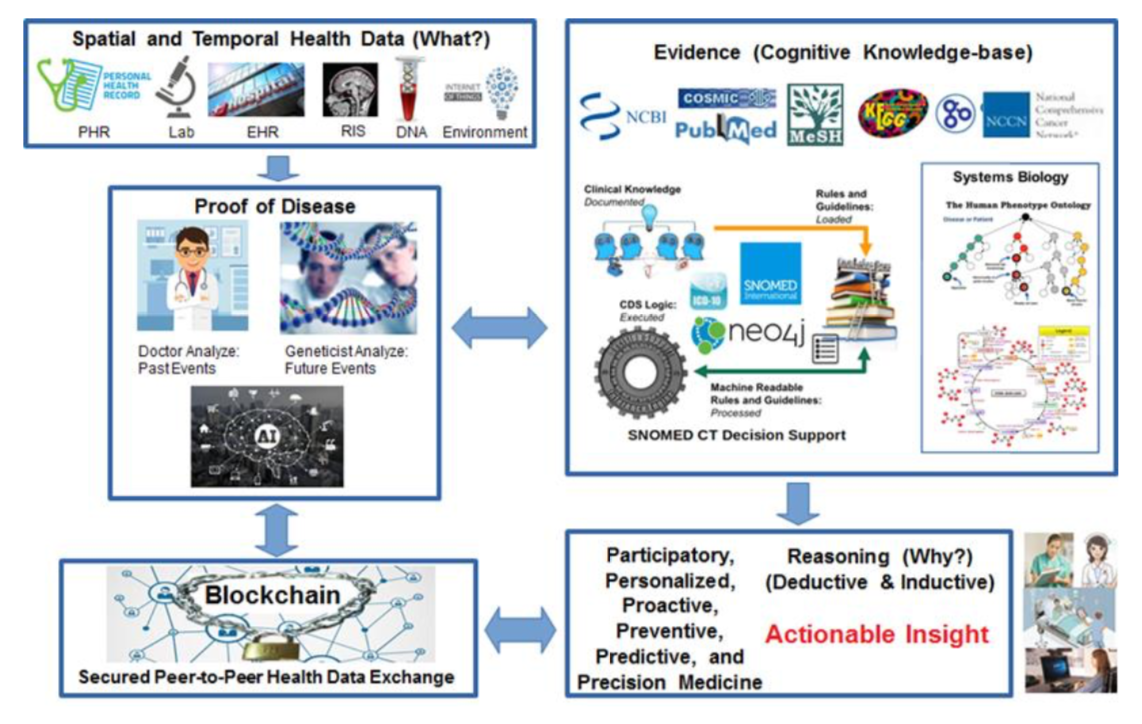
\includegraphics[width=1\textwidth]{images/example_software_architecture.png}
	\caption{Example software architecture cf.\autocite{talukder} pp.260}
	\label{example_software_architecture}
\end{figure}

What is more, there is a medical miner which validates every transaction, then translates all clinical notes into structured \ac{icd} or \ac{snowmed ct} codes. After that, all codes are stored into a smart contract. During that process, a medical expert validates whether the current onset matches any clinical pathway. 
Finally, medical experts discuss in a proper medical consensus if the data is useful for an accurate diagnosis and public health.

\subsection{\ac{soa} for big data applications in the cloud}
The state-of-the art architecture for any project is \ac{soa} and has many advantages, such as flexibility, agility, process orientation, time-to-market and innovation\footnote{cf.\autocite{zimmermann} pp.130}. What is more, \ac{soa} is convenient for cloud computing since it is ready for extended service models.
Figure \ref{esarc_example} shows the architecture 'ESARC', developed by Zimmermann et al.\footnote{cf.\autocite{zimmermann} p.132}. It helps to cluster, classify, examine, compare, evaluate quality and optimize enterprise architectures. As depicted by figure \ref{esarc_example}, there is a link between enterprise and business information and design for supporting strategic initiatives. What is more, ESARC enables integration capacities for \ac{IT} management, software engineering, service and operations management as well as process improvement initiatives.

\begin{figure}[htbp]
	\centering
	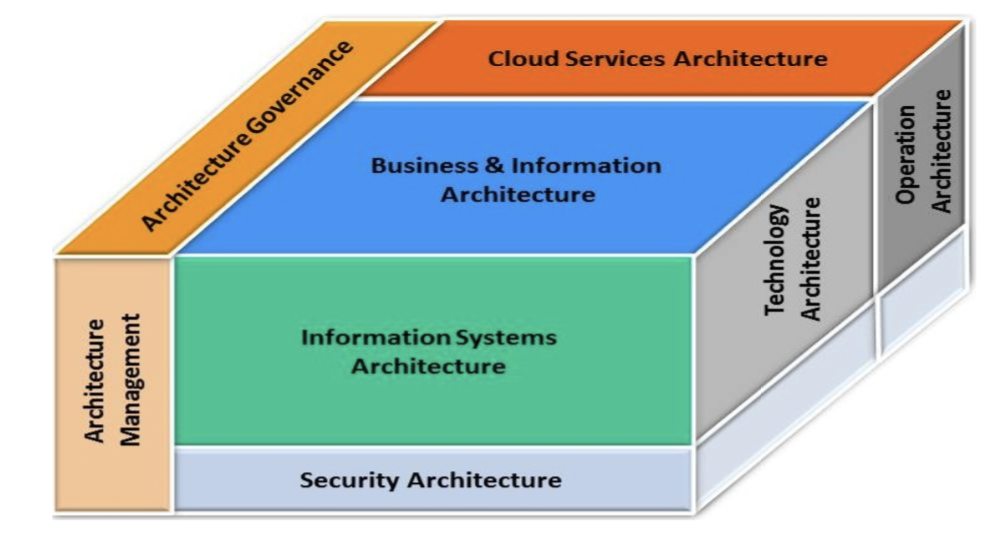
\includegraphics[width=1\textwidth]{images/esarc_cube.png}
	\caption{\ac{esarc} as an example for big data architecture cf.\autocite{zimmermann} pp.133}
	\label{esarc_example}
\end{figure}

As can be seen in figure \ref{esarc_example}, metamodels are used to define model elements in architectures. They relate architectural elements to ontologies which represent a common vocabulary for enterprise architectures.
Zimmermann et al. recommend that operations of tasks and entity services should not have any knowledge about their process or interactive usage context \footnote{cf.\autocite{zimmermann} pp.133}. Instead, task service operations should be independent from users and sessions and should only implement business functionality.

\begin{figure}[htbp]
	\centering
	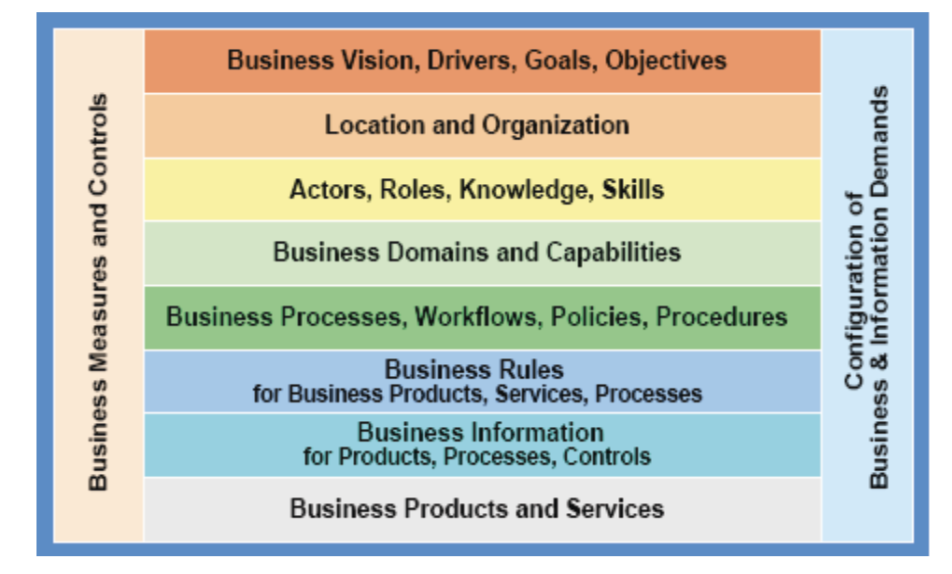
\includegraphics[width=1\textwidth]{images/esarc_business.png}
	\caption{\ac{esarc} business and information reference architecture cf.\autocite{zimmermann} pp.134}
	\label{vp_architecture}
\end{figure}

Figure \ref{vp_architecture} shows a more detailed view of 'ESARC', the procedural framework for architecture assessment processes and questionnaire design. On top of the graphic, with orange background, there are business vision, drivers, goals and objectives. To be more precuse, architecture governance has the goal to manage activities such as plan, define, enable, measure, control and sets rules for architecture complicance to internal and external standards. 

\paragraph{Actors in cloud computing}
According to Zimmermann et al., the main actors in cloud computing are cloud consumers, providers, auditors and broker \footnote{cf.\autocite{zimmermann} pp.133}. In general, all \ac{soa} services are cloud services and follow a reference architecture: 'Jericho-Security-focused Service-oriented Reference architecture for cloud computing'. Thereby, management perspectives from \ac{itil} and \ac{togaf} standards are integrated.

\section{Medical Documentation Apps}

\subsection{Overview: Smartphone apps to support self-management of hypertension}
There exist many different self-management applications for patients who suffer from hypertension. Generally, these self-management programs are likely to be effective if they track the behaviour of their users\footnote{cf.\autocite{alessa} p.1}. This means that medical self-management applications should be supported by theory-based interventions, such as identifying the target behaviour and strategies of behavioural changes needed to achieve desirable health outcomes.
\paragraph{Key functionalities}
As depicted by Alessa et al., important functionalities of medical self-management applications are stress management, communication with \ac{hcp}, self-monitoring abilities (e.g. portrayed in graphs or tables), reminders, automatic feedback and educational information.
\paragraph{\ac{bct}}
Alessa et al. describe important functionalities during the development of medical self-management applications: \ac{bct} which form a theoretical domain framework. These recommendations include:

\begin{itemize}
\setlength\itemsep{-0.5em}
  \item behaviour regulation
  \item knowledge 
  \item goals
  \item memory attention and decision process
  \item beliefs about consequences
\end{itemize}

In their study, Alessa et al. studied that many applications supporting self-management of hypertension have similar functionalities\footnote{cf.\autocite{alessa} p.2}.
Besides these findings, Alessa et al. state that privacy and security is an important issue in many health applications and that these are not available in 35\% of all applications. Moreover, it should be ensured that users are able to make fully informaed decisions by equipping the applications with skills and information necessary to scrutinize the privacy and security policies. This is due to the lack of knowledge and experience of many users in privacy concerns which can be seen in the social media\footnote{cf.\autocite{alessa} p.3}.

\subsection{Blood pressure monitoring in cardiovascular medicine and therapeutics}
As mentioned above, many medical applications are developed for self-monitoring\footnote{cf. p.4ff.\autocite{white_blood_2007}}. These bring many advantages and disadvantages. On the one hand, home blood pressure measurements are representative of natural environment and can show the response to antihypertensive medication. Furthermore, it is an easy and cost-effective way for obtaining a large number of readings. 
On the other hand, the measurement monitors might be too inaccurate and only a few devices have been subjected proper validation and failed tests.
White et al. mention three different monitors for home measurements: arm, wrist and finger monitors. Moreover, multiple readings, e.g. two or three per day are recommended \footnote{cf. p.23ff.\autocite{white_blood_2007}}

\paragraph{Influence factors of hypertension}
There are multiple factors which increase blood pressure, such as age, gender, environmental factors, smoking, alcohol, medication, caffeine, stress and talking.
To be more precisely, e.g. women have lower blood pressure than men or age increases the blood pressure\footnote{cf.\autocite{white_blood_2007} pp.9}. Environmental factors describe the influence of winter or summer terms on the blood pressure values. In winter, it is possible that blood pressure values increase up to 5 mmHg. Besides, the time of date can also influence measurements. For instance, it is recommended that patients take readings in the early morning and night. And there are differences between multiple systolic measurements whereas diastolic measurements stay nearly the same. But the most important fact, stated by White et al. is that summer and exercice dicrease the blood pressure measurements\footnote{cf.\autocite{white_blood_2007} pp.9}.

\paragraph{Future trends in blood pressure measurements}
As explained by White et al., it is very useful to have all readings available in an electronic form and to use these together with telemonitoring \footnote{cf.\autocite{white_blood_2007} pp.31}. In detail, the readings could be transferred automatically to the health care provider. This can help to facilitate the communication between physician and patient in an easy way so that they could form virtual hypertension clinic.

\subsection{Social web and use cases for medical apps}
As stated by Lupton et al.\footnote{cf.\autocite{lupton_apps} p.607} the current technical 'era' we are living in is the web 2.0 or social web. Social web includes sharing health and medical information with each other, e.g. patients and caregivers write about experiences and the individual health status. Often, the aim of these social webs is to control the health status by using online information and imaging.
Conforming to Lupton et al.\footnote{cf.\autocite{lupton_apps} p.608}, in healthcare projects, big data can be used to generate knowledge about healthcare, health behaviours and disease patterns. Such applications can assist in calculating diagnosis, identifying risks, facilitating health, fitness self-tracking as well as patient self-care regimes.
As reported by a study which surveyed American doctors\footnote{cf.\autocite{lupton_apps} p.610}, medication interaction apps are the first most-used and diagnosis apps the second most used category of apps.
Moreover, pregnancy apps offer greater opportunities, such as that women can engage obsessive self-surveillance because of producing detailed data, such as heart rates, in real-time\footnote{cf.\autocite{lupton_apps} pp.614}. Pursuant to Lupton et al., the future potential of medical application lies in systems which enable lay people to access medical information (such as the electronic medical record) that was previously only available to healthcare practitioners or students.

In another article, Lupton et al. reported that the potential lies in automation of news or notifications which can be personalized or targeted so that doctors could contact patients directly to remind them to adhere to their tratment programs\footnote{cf.\autocite{lupton_mhealth} pp.229}.
A further example of medical applications are 'smart pillboxes' for patients suffering from diabetes\footnote{cf.\autocite{lupton_mhealth} pp.232}. 'Smart pillboxes' are wireless devices that remind patients to take their medication and alert a doctor if the patient had failed to conform to their medication regimen.
Continuing, \ac{m-health} technologies have a feedback, also called cybernetic mechanism in that they react with their users as opposed to passively provide information. To give an example, modern prosthesis or technological extensions of the body are a kind of cybernetic mechanism\footnote{cf.\autocite{lupton_mhealth} pp.234}. 
A big part of today's medical applications are surveillance systems in order to record and monitor cases of illnesses, such as obesity or infections\footnote{cf.\autocite{lupton_mhealth} pp.235}. These records might be useful to early detect epidemiological changes in the disease pattern. To give an example, 'individual medical encounters' which are conducted online enable doctors to flexibly practice personalized surveillance over each of their patients. At this point, another term occurs: 'surveillance knowledge' which refers to the digital data produced in the surveillance and can be useful for the individuate users.

\paragraph{Blockchain solution for accurate medical decisions}
As stated by Talukder et al. a significant amount of today's diagnosis in \ac{ncd} is erroneos or unwanted\footnote{cf.\autocite{talukder} p.263}. The term \ac{ncd} implicates disease caused by an unheallthy lifestyle, the proper environment or genomic causes over a long time and come up with confusing signs and symptoms.
Talukder et al. mention 'P6'-Medicine which describes medicine using six adjectives starting with the letter 'p': medicine needs to be participatory, personalized, proactive, preventive, predictive, precision medicine.
As a requirement list for health data, Talukder et al. describe important features as follows: 

\begin{itemize}
\setlength\itemsep{-0.5em}
  \item secured (the anonymity, privacy, confidentiality of health data must be approved)
  \item systems which provide health data must have a zero down-time 
  \item the integrity of the health data must be ensured
  \item the systems must be ubiquitous which implies an unlimited availability
  \item machine understandable (all health data should be conform to international standards and should be able to be distributed over multiple systems)
  \item health systems should be resistant against fraudulent hacking
\end{itemize}

\section{Chatbots} 

\subsection{The potential of chatbots}
The main advantage of chatbots is to provide a 24-hour customer service with personalized interaction and no waiting time\footnote{cf.\autocite{akhtar} pp.297}. 
Besides, the data retrieval from conversations with chatbots provides many possibilities. To be more precise,  modelling, profiling, analyzing and understanding users becomes increasingly important in many different indrustries and count as key to success in todays data driven world. 
Akhtar et al. analyzed chat conversations between customers and the chatbot of a telecommunication company in order to find out the user's topics of interest and how to satisfy users. As described by Akhtar et al., the tests of the chatbot were splitted into different activities, such as text mining techniques (feedback comments), event sequence analysis, frequent term extraction, analysis of bigrams/trigrams. 
During data preprocessing, Akthar et al. used the following methods:
\begin{itemize}
\setlength\itemsep{-0.5em}
  \item[1.] corpus generation
  \item[2.] eliminating extra white space
  \item[3.] stopwords removal
  \item[4.] tokenizing
  \item[5.] stemming
  \item[6.] creating term-document matrices
\end{itemize}

The main challenges during the data analysis process are data availability, the access to further user information (e.g. contract details or age in order to generate an user model) and the distinction between different user types and different personality structures.

\paragraph{Question Answering Paradigms}
There are several types of conversations which can be designed by building a chatbot\footnote{cf.\autocite{akhtar} p.398}. Generally, there can be distinguished between two different paradigms: information-retrieval based Question and Answering and knowledge-based Question and Answering. The first type describes the mechanism to define short texts as answers to a user's intent. On the opposite, the second type describes how to in natural language. The answers are stored into a full-related database and the conversation works simply with a rule-based method.
\paragraph{Types of dialog systems}
In general, dialog systems can be divided into two kinds of systems. On the one hand, there are task-oriented systems which are appropriate for short conversations and built for a certain purpose. On the other hand, there are non-task-oriented systems which are built for longer and more complex interactions with the purpose of imitating human conversations\footnote{cf.\autocite{akhtar} pp.399}.

\subsection{A deep learning question-answering specialized chatbot for medical students}
During their studies, medical students have to take an exam which is called \ac{osce} where they interact with a 'standardized' patient played by an actor who simulates the symptoms and intents of the patient\footnote{cf.\autocite{zini} p.2}. The aim of this exam is to test and assess the students' abilities and social interaction and diagnosis skills.
Since in practice, there are not many actors who can play a patient's role, Zini et al. developed a virtual patient and chatbot system which works with \ac{nlp} techniques.

Figure \ref{vp_architecture} shows the architecture of the developed system to create a virtual patient. Zini et al. used a \ac{cnn} and \ac{lstm} network in order to learn domain specific word embeddings, sentence embedding and answer selection models.
The embeddings model which is outlined by a red rectangle in figure \ref{vp_architecture} is trained on a corpus of medical documents.
In Figure \ref{vp_architecture}, there is a \ac{nlp} engine outlined by a red rectangle. By using a supervised learning scheme to learn a mapping between question and answering pairs and judgement of correct match, this \ac{nlp} engine should correctly answer questions based on a script.

\begin{figure}[htbp]
	\centering
	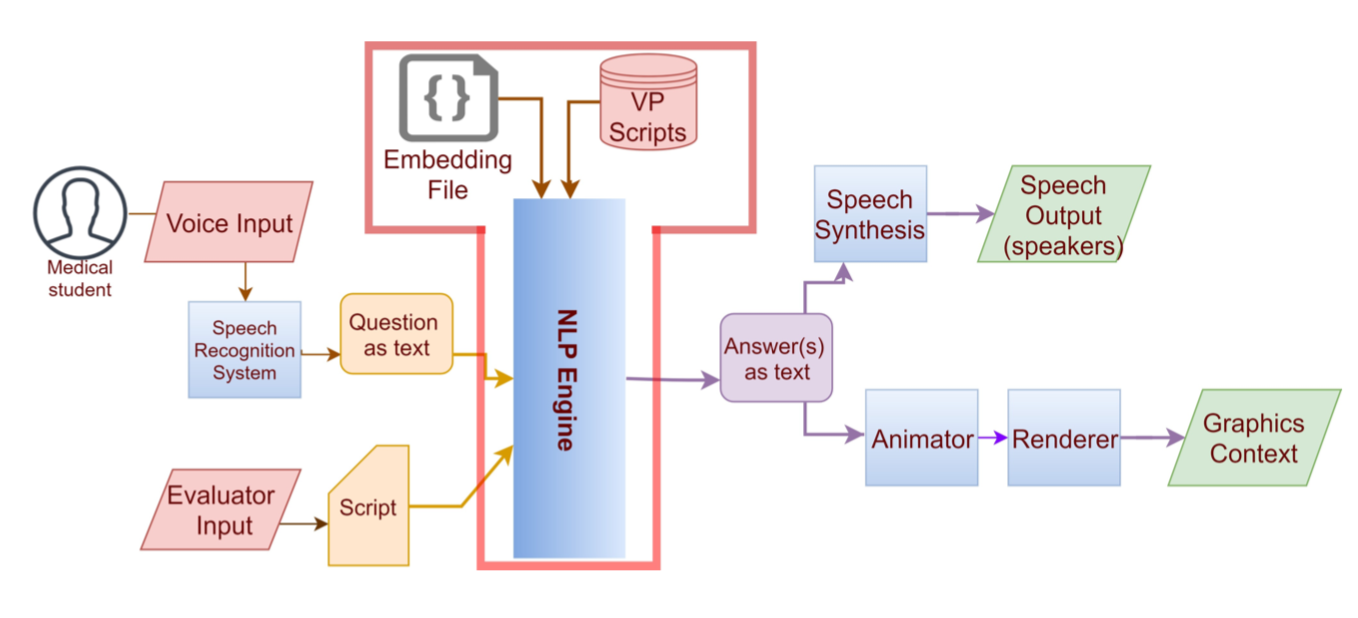
\includegraphics[width=1\textwidth]{images/vp_architecture.png}
	\caption{Virtual patient software architecture cf.\autocite{zini} p.3}
	\label{vp_architecture}
\end{figure}

The aim of the developed system was to create a deep learning framework for answer selection in the medical domain and to create domain-specific word and sentence embedding models. Additionally, a question and answering corpus should be created for \ac{osce}s.

\paragraph{Question and Answering systems}
According to Zini et al. there are two types of question and answering systems\footnote{cf.\autocite{zini} pp.4}. First of all, there is open domain question and answering which uses very specific terminology. Secondly there are restricted domain question and answering systems which are broader in their scope. These are for example insurance-related deep learning question and answering systems which make use of two baseline models: \ac{bow} and \ac{ir} model. 

\chapter{Analysis and Development}

First of all, the developed chatbot includes information about blood pressure and was built to remind patients of their measurements. Secondly, based on the measured data, analysis can be done in order to react earlier to outliers. Thirdly, a generated report is sent to the doctor via email so that he can get more insights about the blood pressure values of his patients and can improve the treatment.
One of the main challenges during development was the process of providing information about the disease to the patient. Is it possible to include information about different types of blood pressure into the automated conversation with a chatbot? Or does it overwhelm the conversation's use case? Is it useful to let the user ask questions like: 'What are the different types of hypertension? Am i a high-risk patient?' 
Or should these information be provided as a video or a simple web page with long articles to read? Might the patient or user be aborred after a while of talking to a chatbot who only knows answering his questions in the same way?
Of course, a chatbot can be developed in a more intelligentway to never provide the same answer and to answer more precisely to a users' intent. But this requires a lot of training and testing. 
For that reason, in the first version of this chatbot, five simple intents and dialogs have been designed and implemented with the focus of the instructions to measure correctly and regularly. 
In a second or third version, it is possible to focus more on the improvement of providing information about the disease (by not doing this in the style of question and answering).

\section{Experimental set-up}

\subsection{Software architecture}

Figure \ref{architecture_0102} gives an overview of all developed components. Quite above, there is the Watson Assistant instance, running in the IBM Cloud. Beneath Watson Assistant, a NodeJS server opens the session and sends messages from the client to the Assistant and backwards. The NodeJS server connects the cloud and the frontend by implementing \ac{http} requests and responses. Finally, there is the AngularJS application running locally and creating a \ac{JSON} reporting file every few minutes. This reporting file includes all messages, with the user from whom it was send and a timestamp. It can be used to analyze the data and to create profiles of the patients.

\begin{figure}[ht]
	\centering
	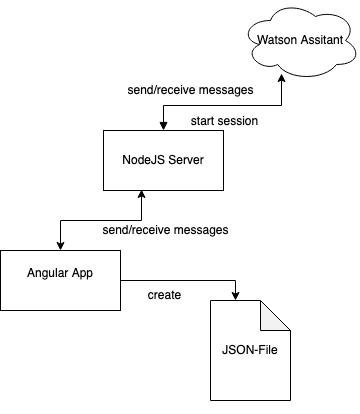
\includegraphics[width=1\textwidth]{images/architecture_0102.png}
	\caption{Architecture diagram of developed system}
	\label{architecture_0102}
\end{figure}


\subsection{Development of Watson Assistant Dialog}

\paragraph{Intent model}

The chatbot was built according to the webpage of "Deutsche Hochdruckliga", a german organization for patients who suffer from hypertonia\footnote{cf.\autocite{hochdruckliga}}. 
To better understand the users and patients a basic intent model with four intents was developed. 
The four intents include 

\begin{center}
\begin{tabular}{ |c|c| } 
\hline
Intent & User input  \\
\hline

\multirow{4}{4em}\\
Definition of hypertonia  & What is hypertonia?  \\ 
Curses of hypertonia & What are the implications or curses of hypertonia? \\ 
Blood pressure measurement &  I am measuring my blood pressure.\\ 
Measurement tutorial & How should i measure my blood pressure? \\ 
\hline
\end{tabular}
\end{center}
  
These four intents were used to define and develop four typical dialogs, displayed in figure \ref{dialog_diagram_01}, \ref{dialog_diagram_02}, \ref{dialog_diagram_03} and \ref{dialog_diagram_04}.

\begin{figure}[h]
	\centering
	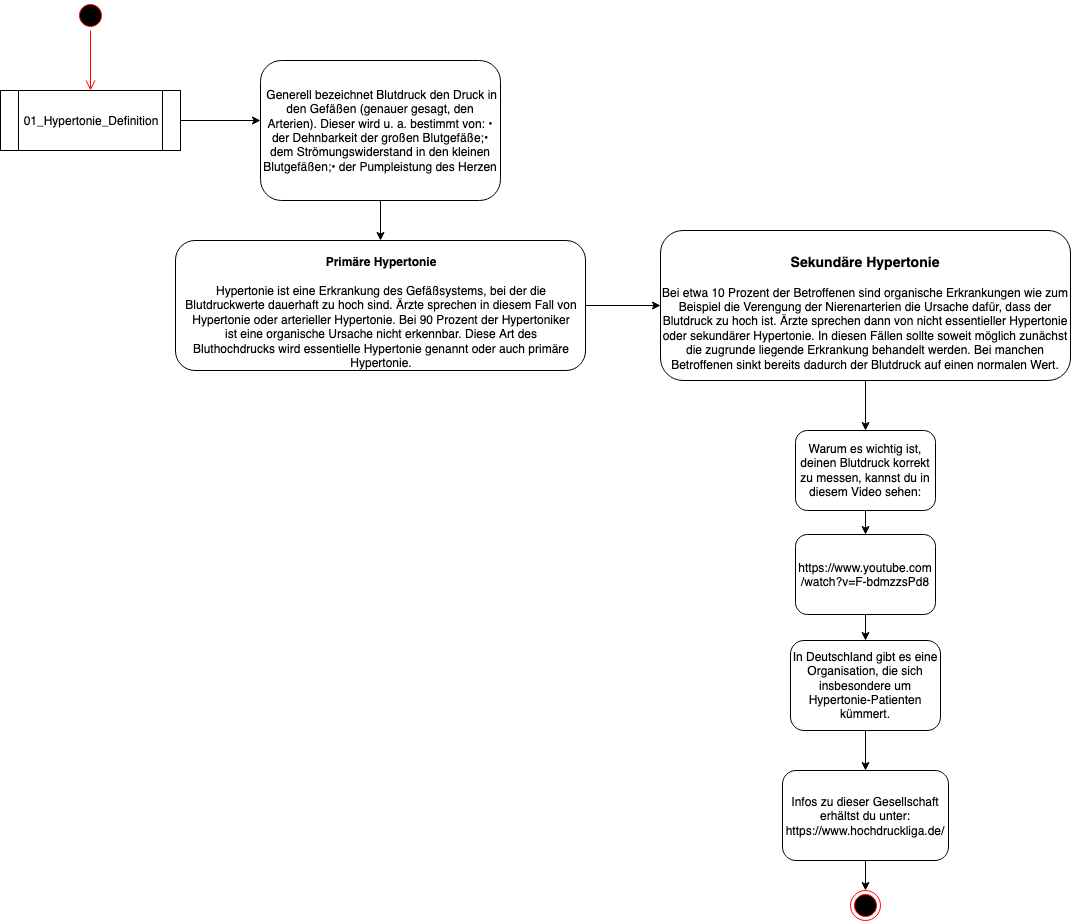
\includegraphics[width=1\textwidth]{images/01_Hypertonie_Definition.png}
	\caption{Dialog diagram: definition of hypertonia}
	\label{dialog_diagram_01}
\end{figure}

\begin{figure}[h]
	\centering
	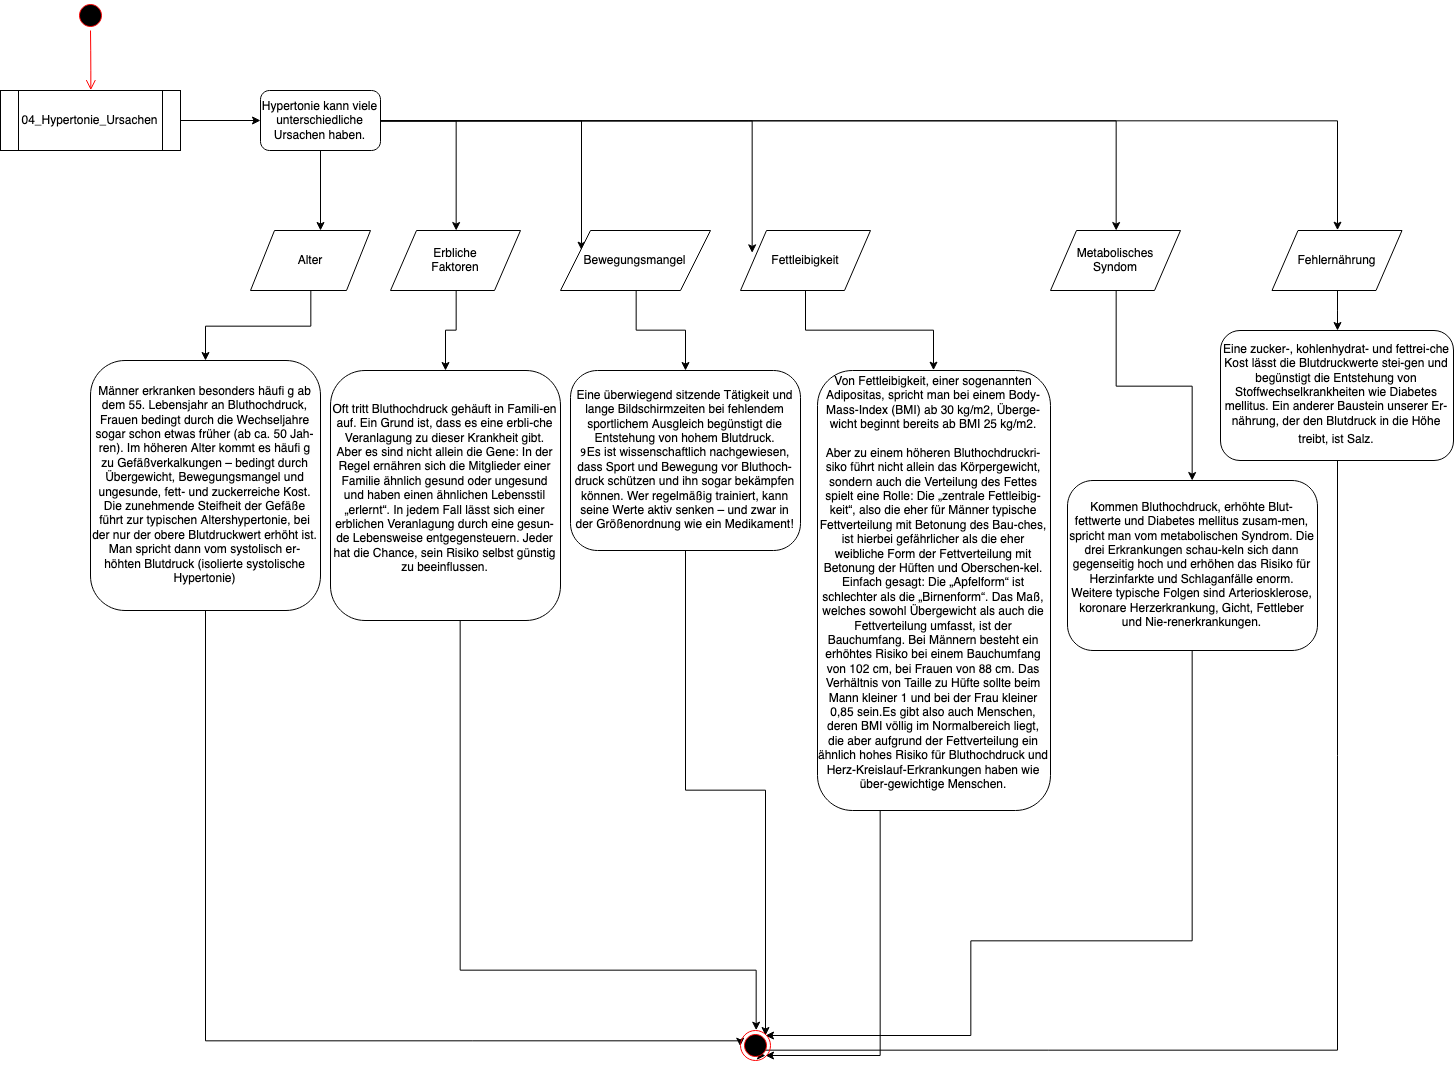
\includegraphics[width=1\textwidth]{images/02_Hypertonie_Ursachen.png}
	\caption{Dialog diagram: curses of hypertonia}
	\label{dialog_diagram_02}
\end{figure}

\begin{figure}[h]
	\centering
	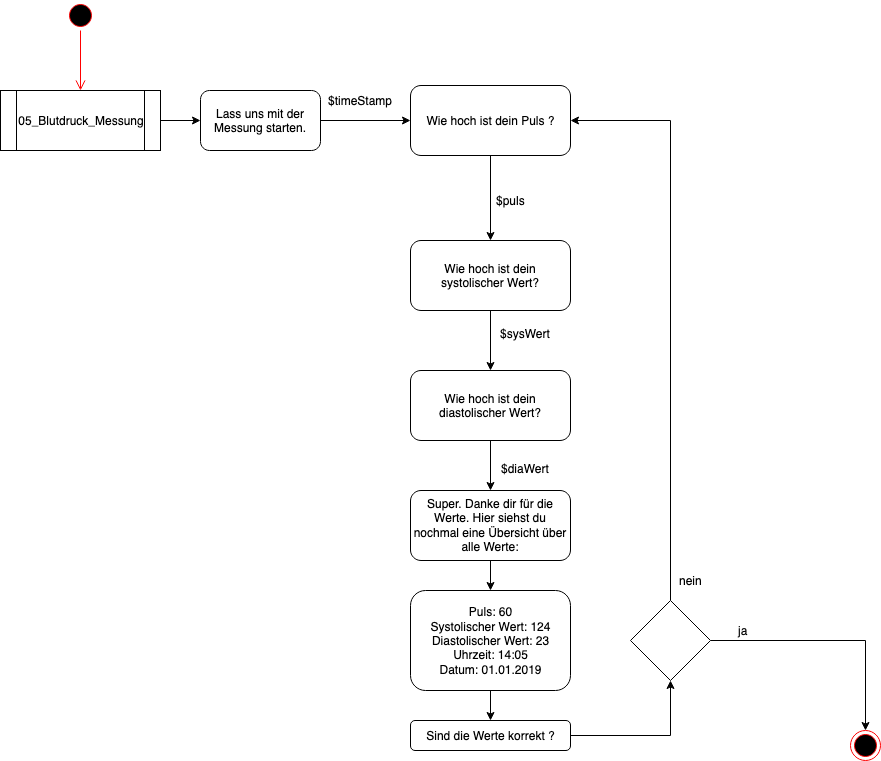
\includegraphics[width=1\textwidth]{images/03_blutdruck_messung.png}
	\caption{Dialog diagram: blood pressure measurement}
	\label{dialog_diagram_03}
\end{figure}

\begin{figure}[h]
	\centering
	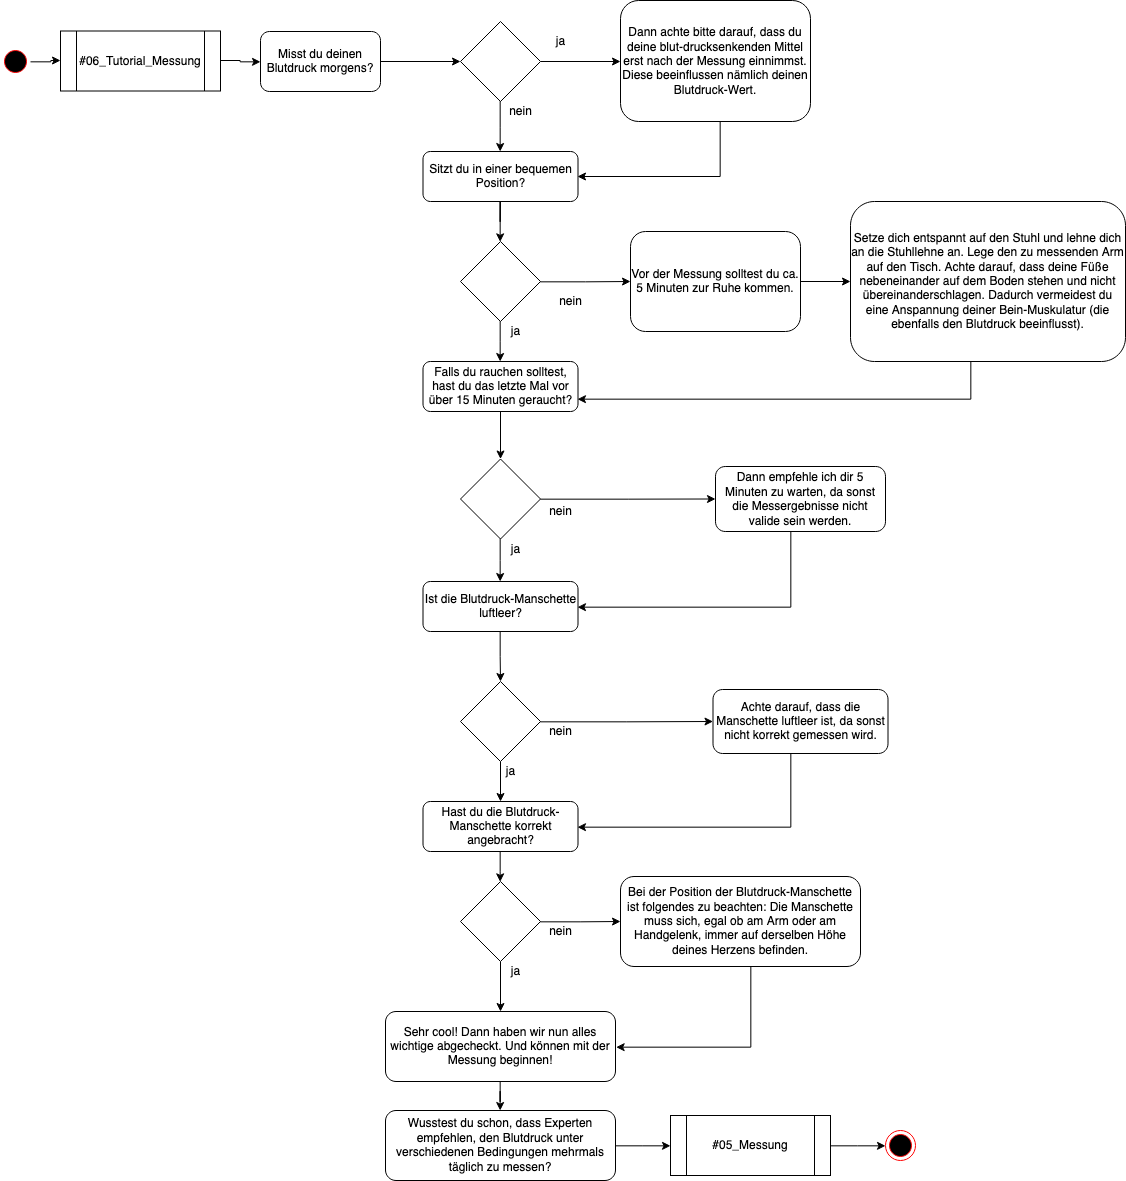
\includegraphics[width=1\textwidth]{images/06_tutorial_messung.png}
	\caption{Dialog diagram: measurement tutorial}
	\label{dialog_diagram_04}
\end{figure}


\paragraph{Watson Assistant implementation}

In the following, the implemented dialog as well as all entities and intents are described. They have been developed according to the Watson Assistant documentation \footnote{cf.\autocite{wa_docu}}.
Basically, 16 entities (see figure \ref{wa_entities}) and 17 intents (see figure \ref{wa_intents}) were defined. Entities give examples of an user's input.
The dialog (see figure \ref{wa_dialog}) includes a welcome node, a concierge node which asks the basic data (e.g. age, gender, height, weight etc.) and starts the tutorial, an additional information node (if the user wants to know more about hypertonia), the measurement node and finally the recommendation of doctors node.

\begin{figure}[ht]
	\centering
	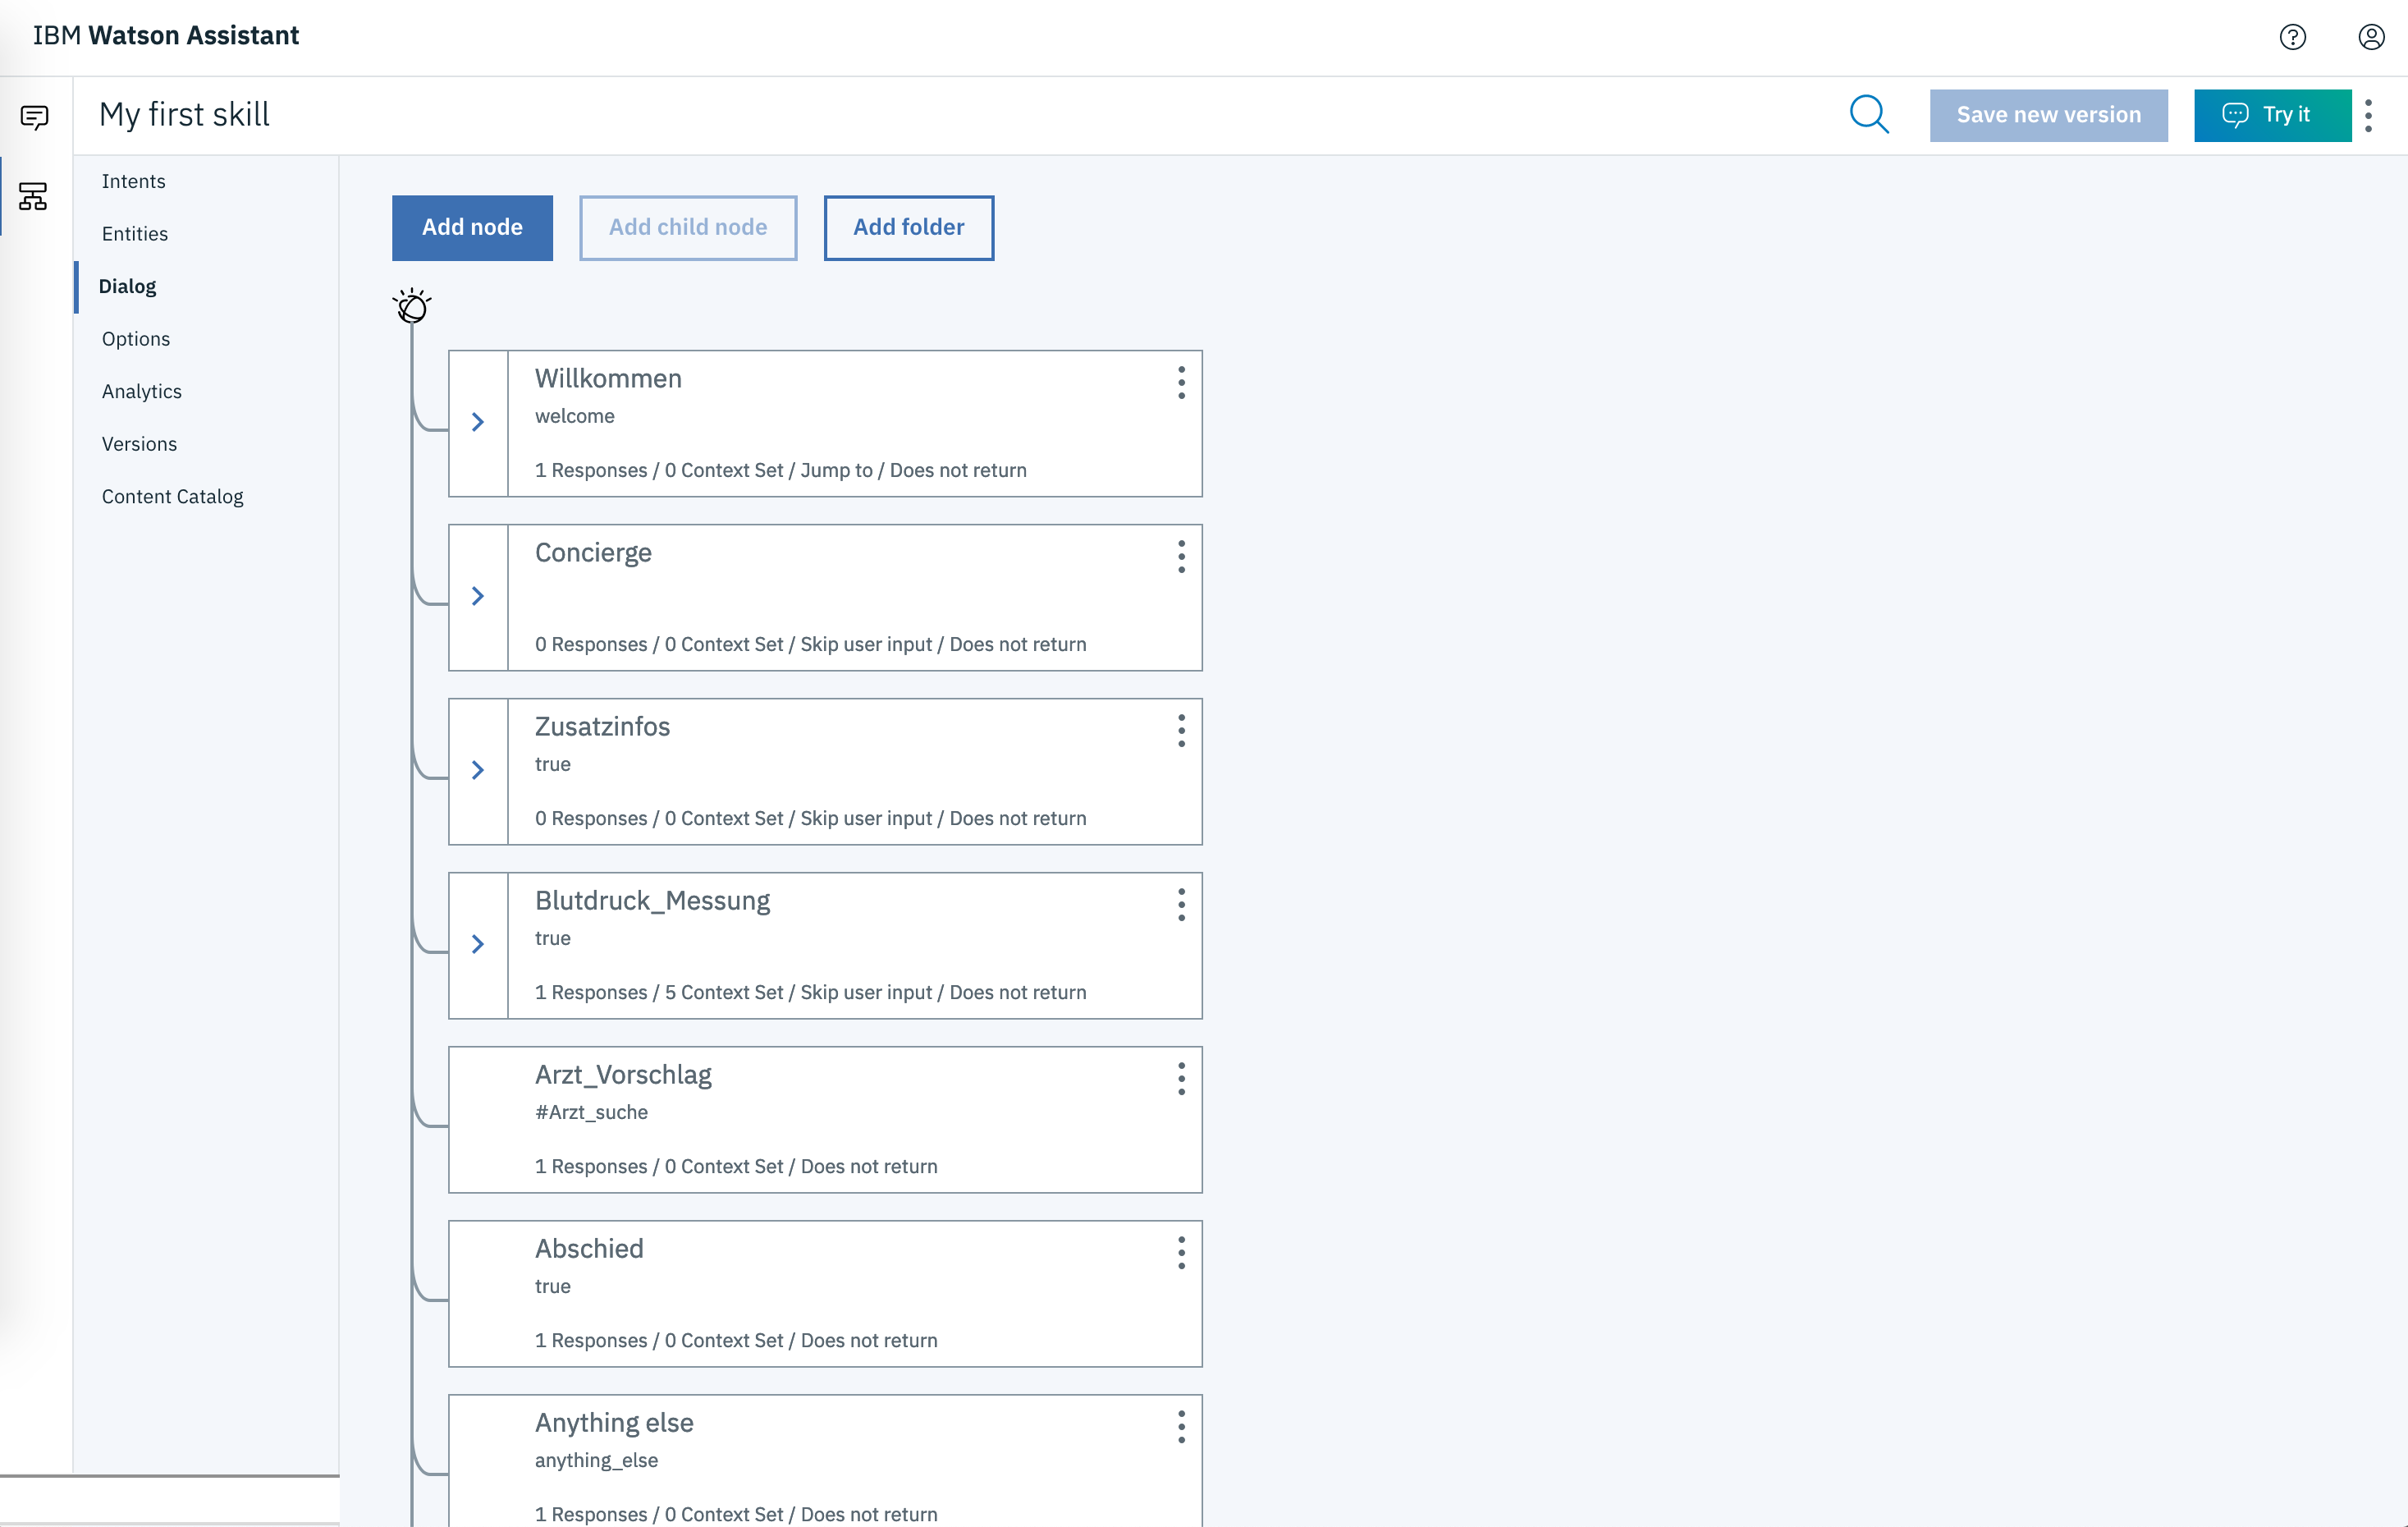
\includegraphics[width=1\textwidth]{images/WA_dialog.png}
	\caption{Watson Assistant dialog}
	\label{wa_dialog}
\end{figure}

\begin{figure}[ht]
	\centering
	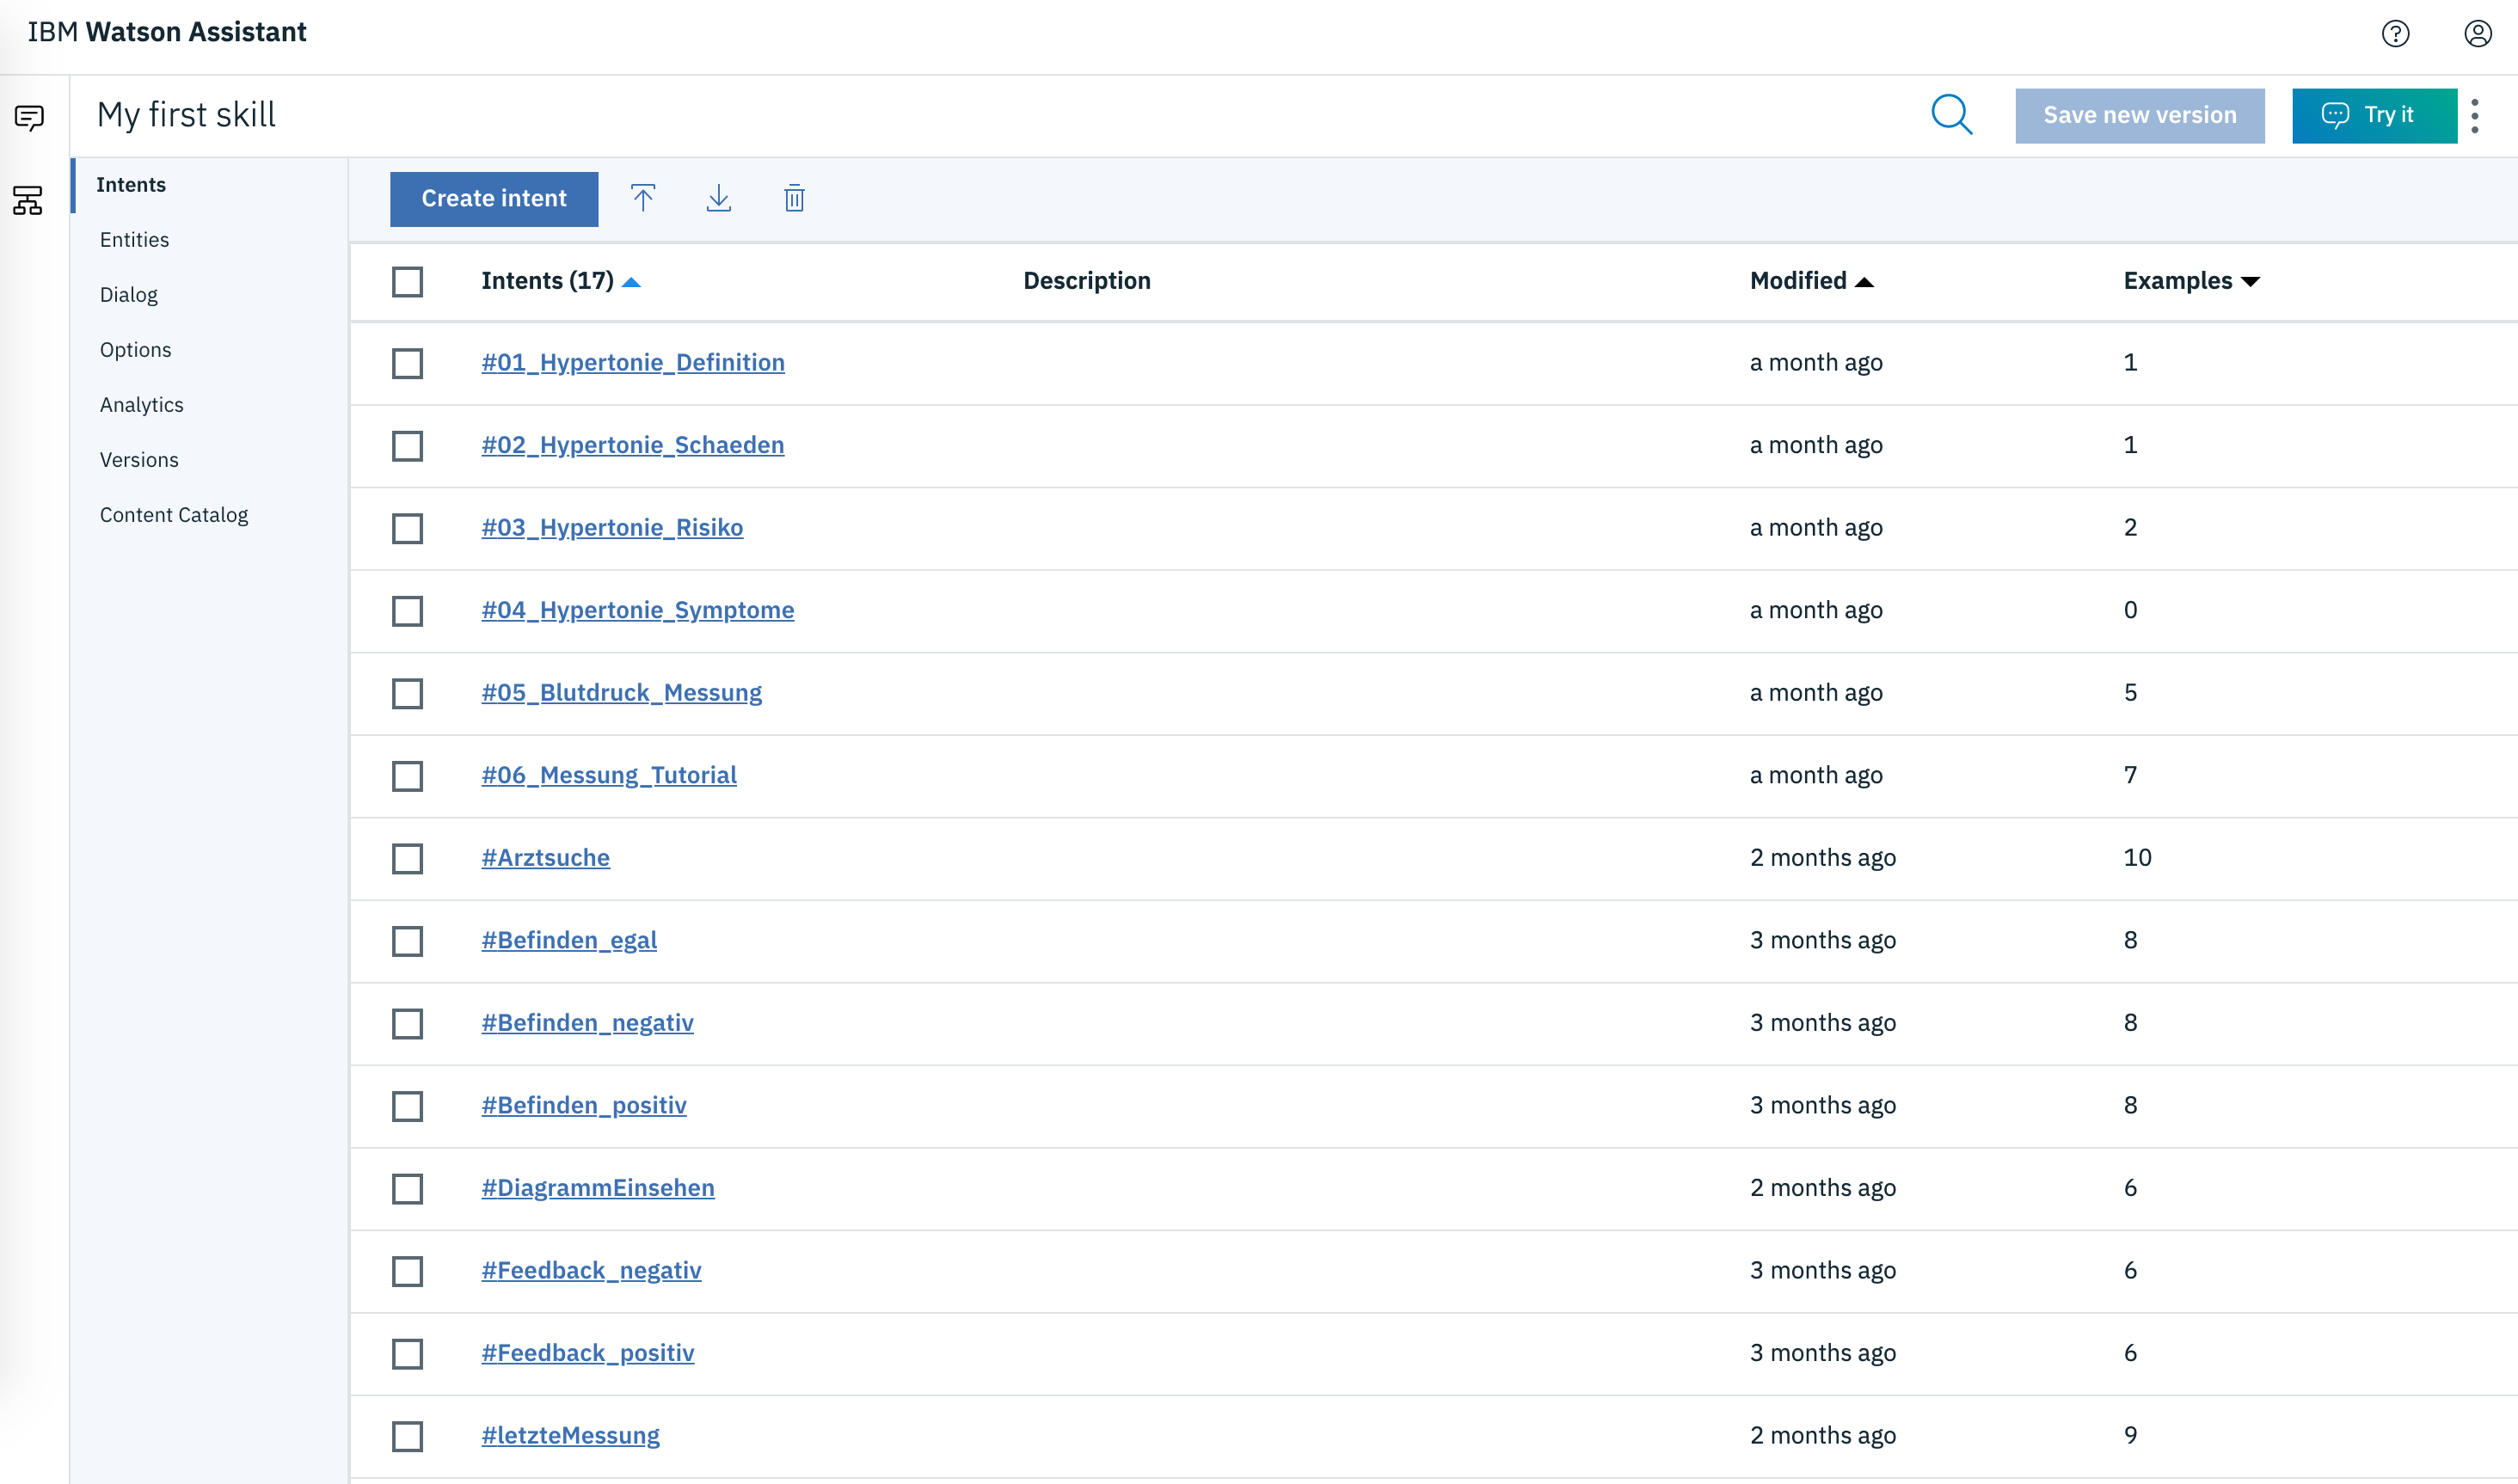
\includegraphics[width=1\textwidth]{images/WA_intents.png}
	\caption{Watson Assistant intents}
	\label{wa_intents}
\end{figure}

\begin{figure}[ht]
	\centering
	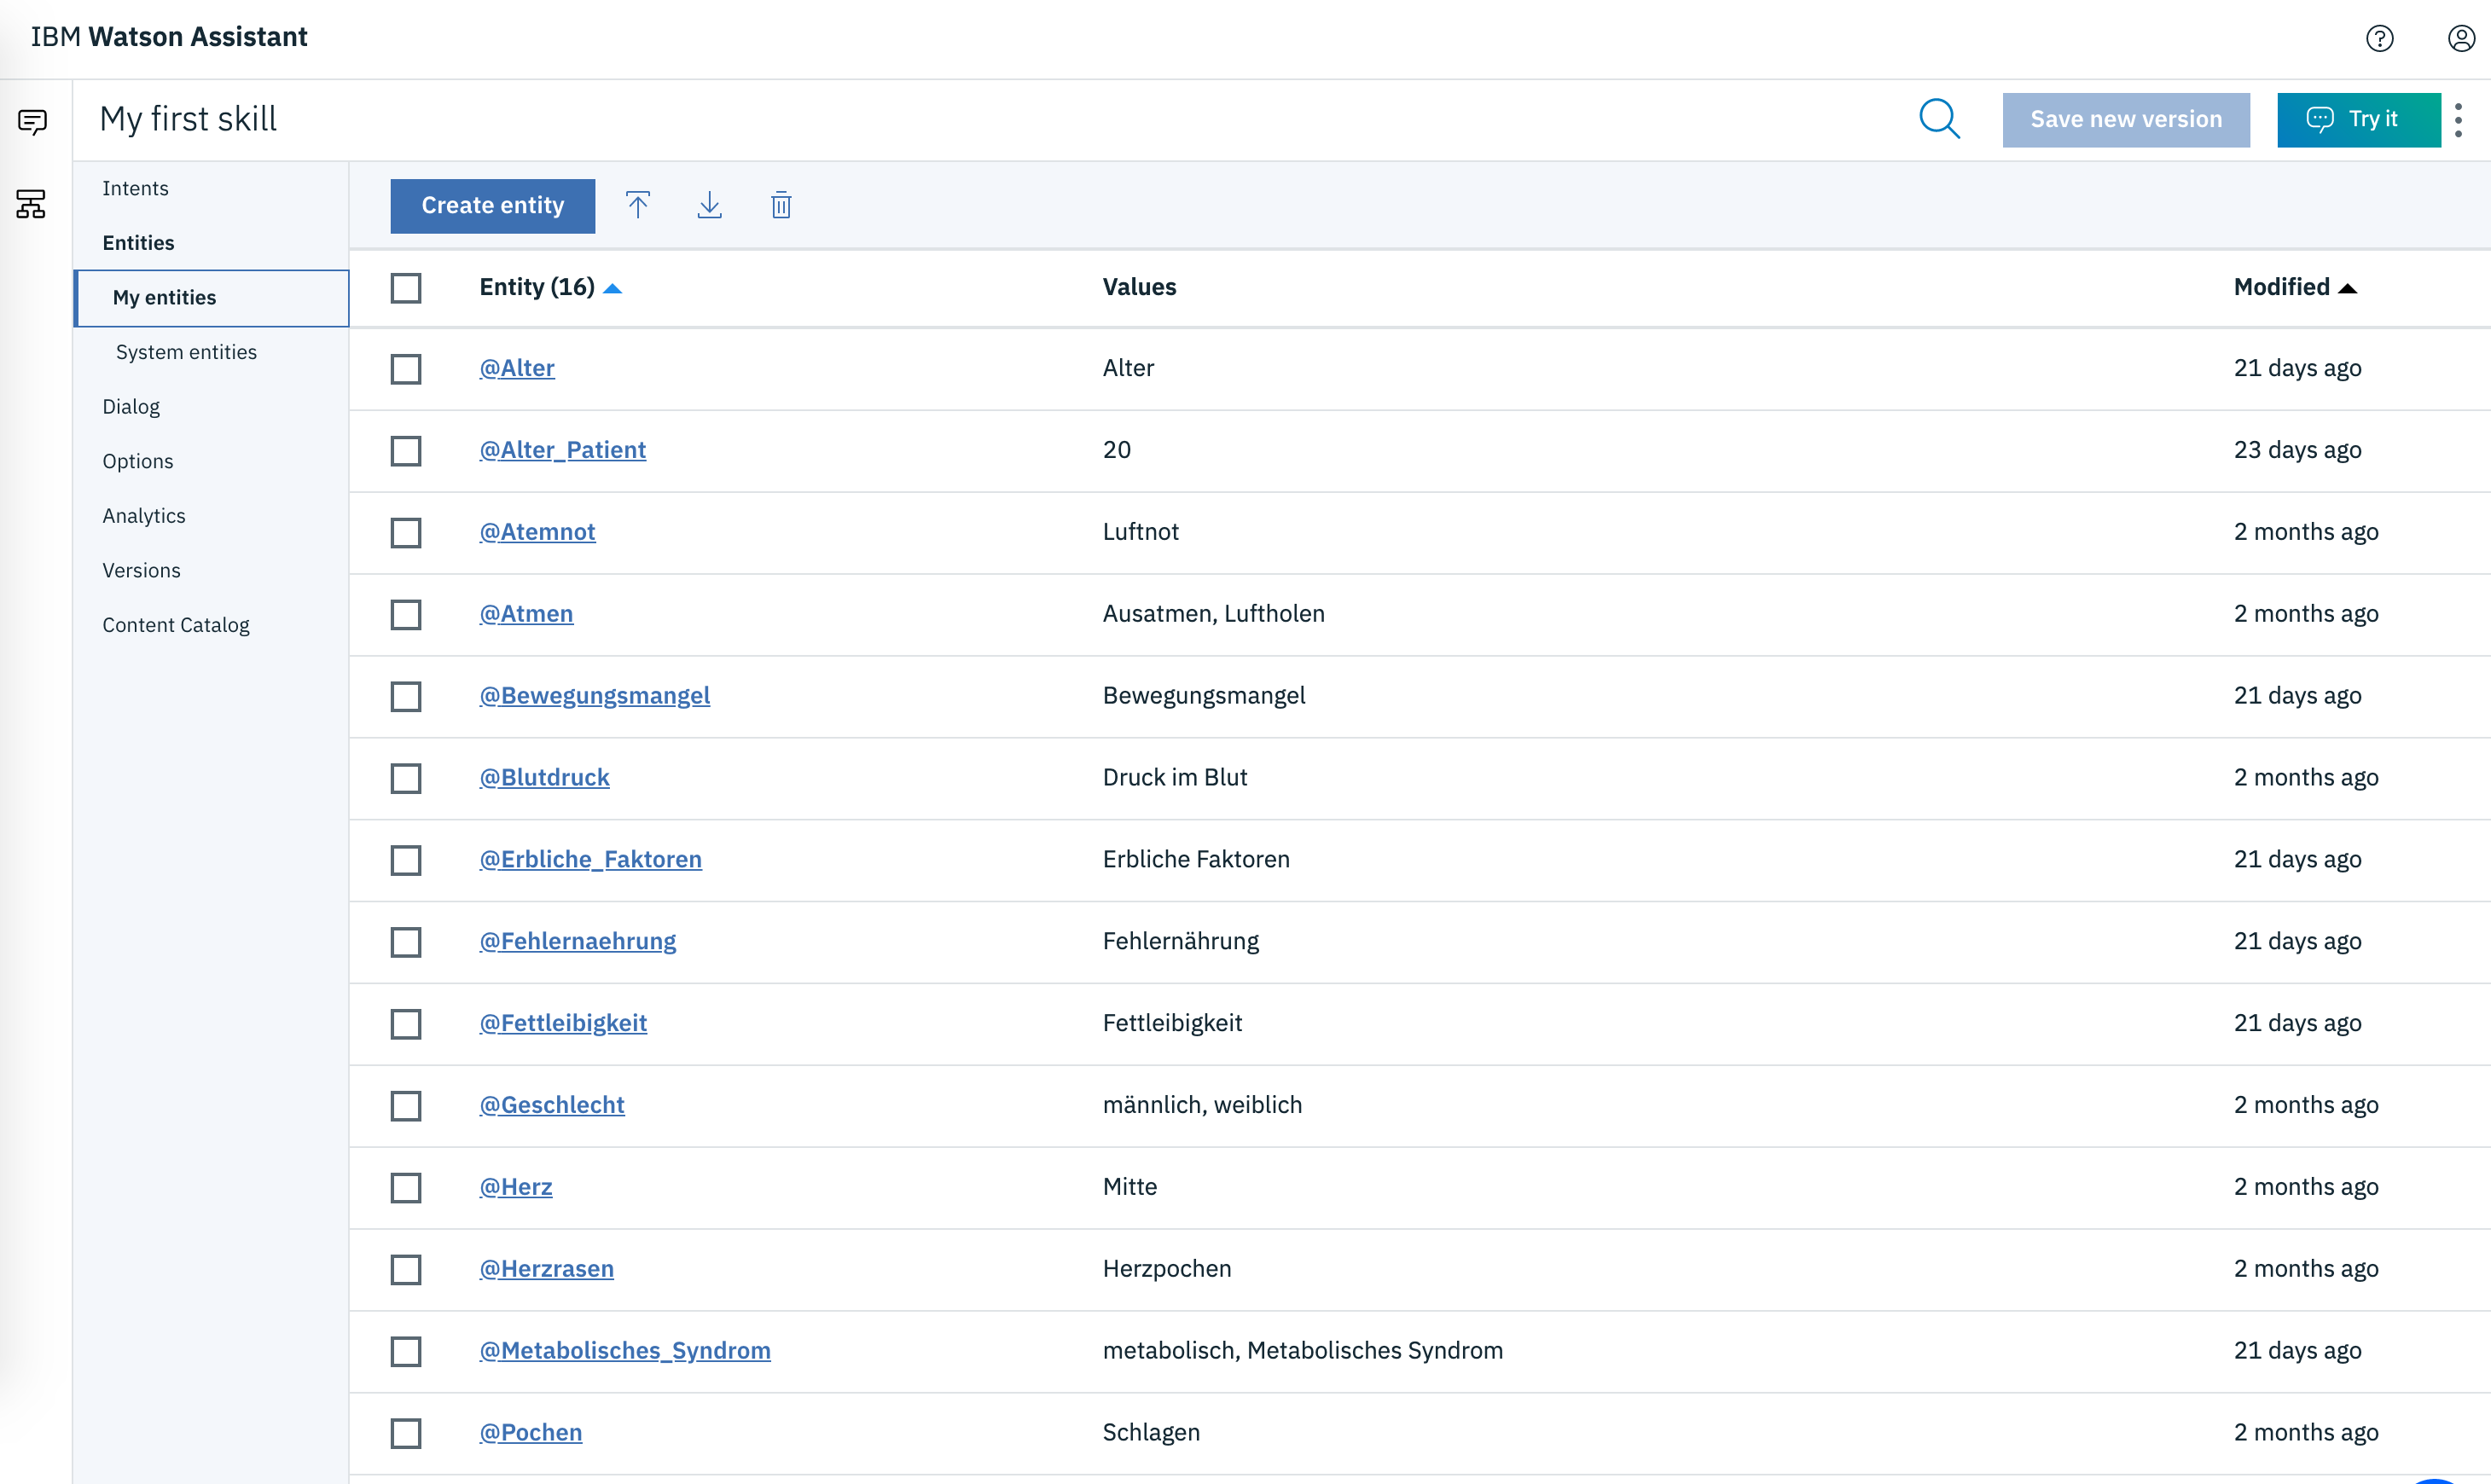
\includegraphics[width=1\textwidth]{images/WA_entities.png}
	\caption{Watson Assistant entitities}
	\label{wa_entities}
\end{figure}

\paragraph{Setup of AngularJS Frontend}

In order to provide a comfortable way to chat and view all retrieved and measured data, a basic angular application was built and run locally (see figures \ref{angular_01} and \ref{angular_02}). Three open source ibraries, such as Nebular\footnote{cf.\autocite{nebular}}, Apache Echarts\footnote{cf.\autocite{echarts}} and Openlayers Maps\footnote{cf.\autocite{openlayers}} were included to the application. Nebular is a Javascript library that has certain themes (e.g. light, dark etc.) and a chat UI (which allows to send messages and different file types such as documents or images or videos). It also allows to send a location by defining longitude and latitude parameters. Generally, it is very handy and useful to fast built up an Angular webpage.
Secondly, Apache Echarts is also a Javascript library which offers a huge variety of diagrams and maps, such as bar, line, pie and other special diagrams (including different animation modes, overlays and tooltips). For the first draft of the frontend, the basic line chart was used to display the weekly, monthly and yearly overview of measured pulse, systolic and diastolic values. But for future use cases, it might be also useful to display other charts of Echarts or maybe tables.
The third Javascript library that was used, is called Openlayers Maps. It is very famous and many projects rather use Openlayers API than Google Places API because their API calls are very expensive. Openlayers Maps has many different modes and overlays. Certain places can be marked by different icons.
All in all, the three described libraries were very well documented and are easy and ready to use after installation, so that the focus could be spent more on developing the Watson Assistant dialog described in the next paragraph.

\begin{figure}[h]
	\centering
	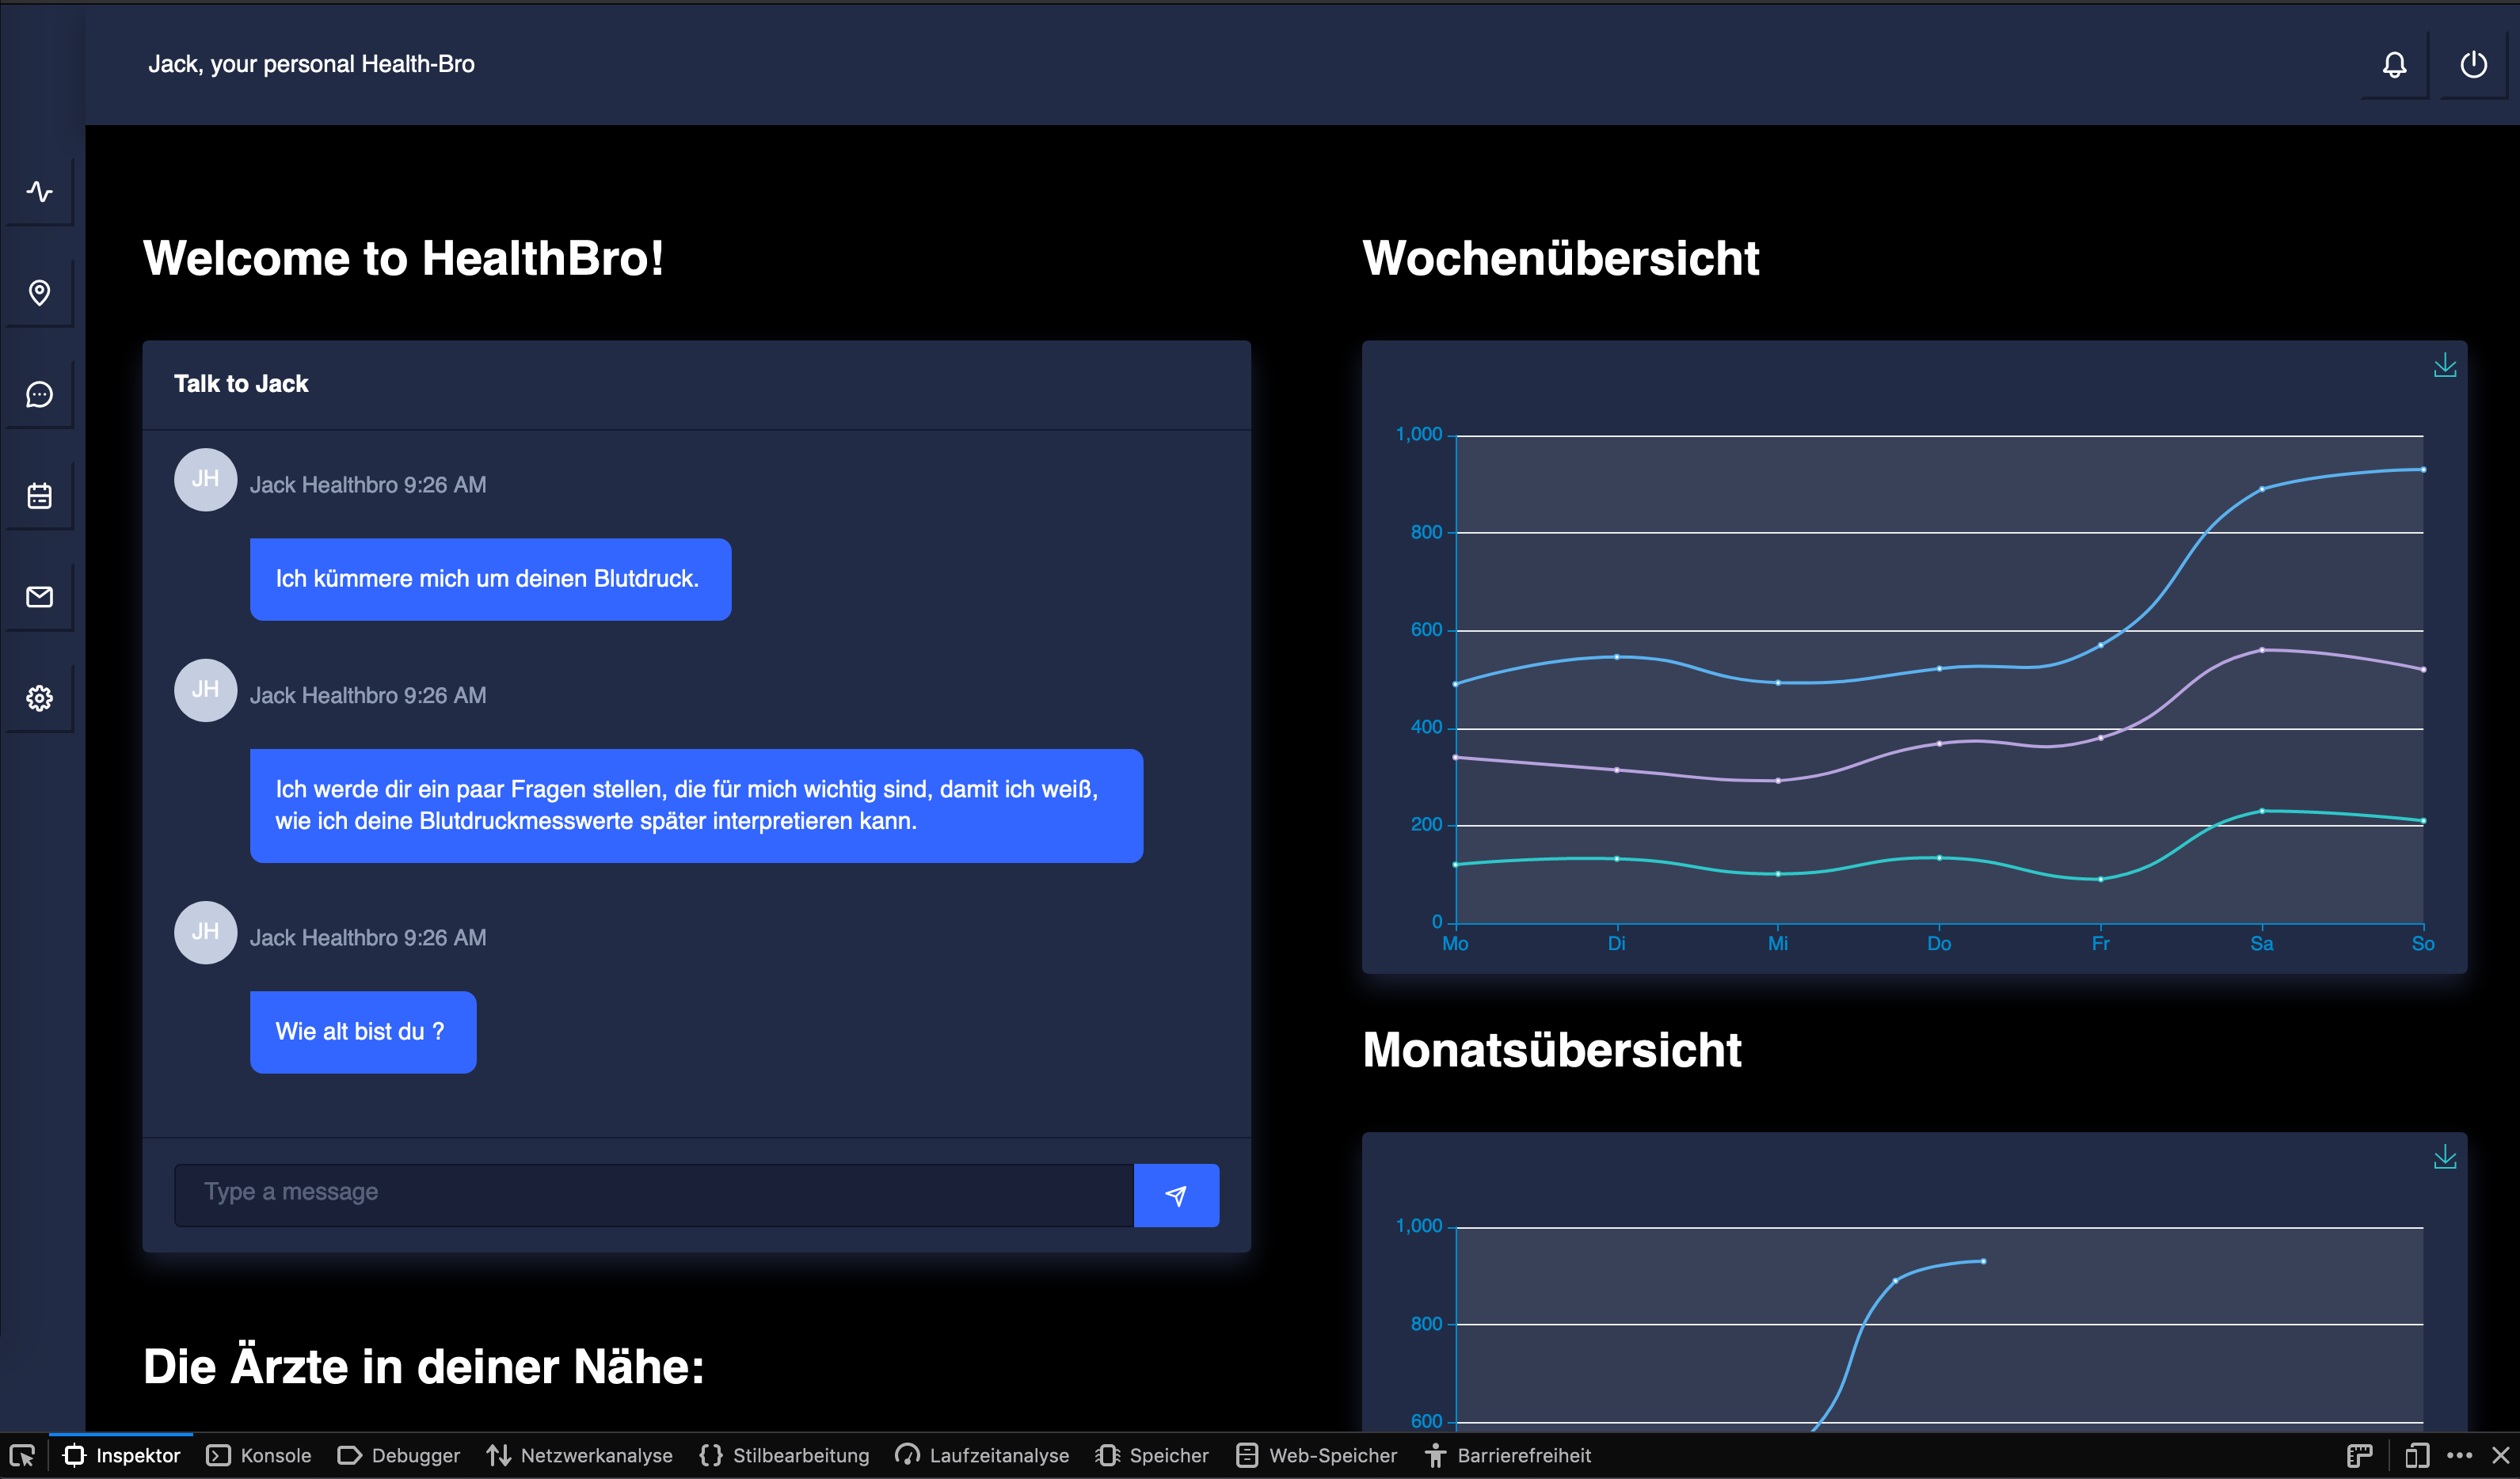
\includegraphics[width=1\textwidth]{images/angular_01.png}
	\caption{Angular Frontend (top page), chat UI and diagrams of measured values}
	\label{angular_01}
\end{figure}
\begin{figure}[h]
	\centering
	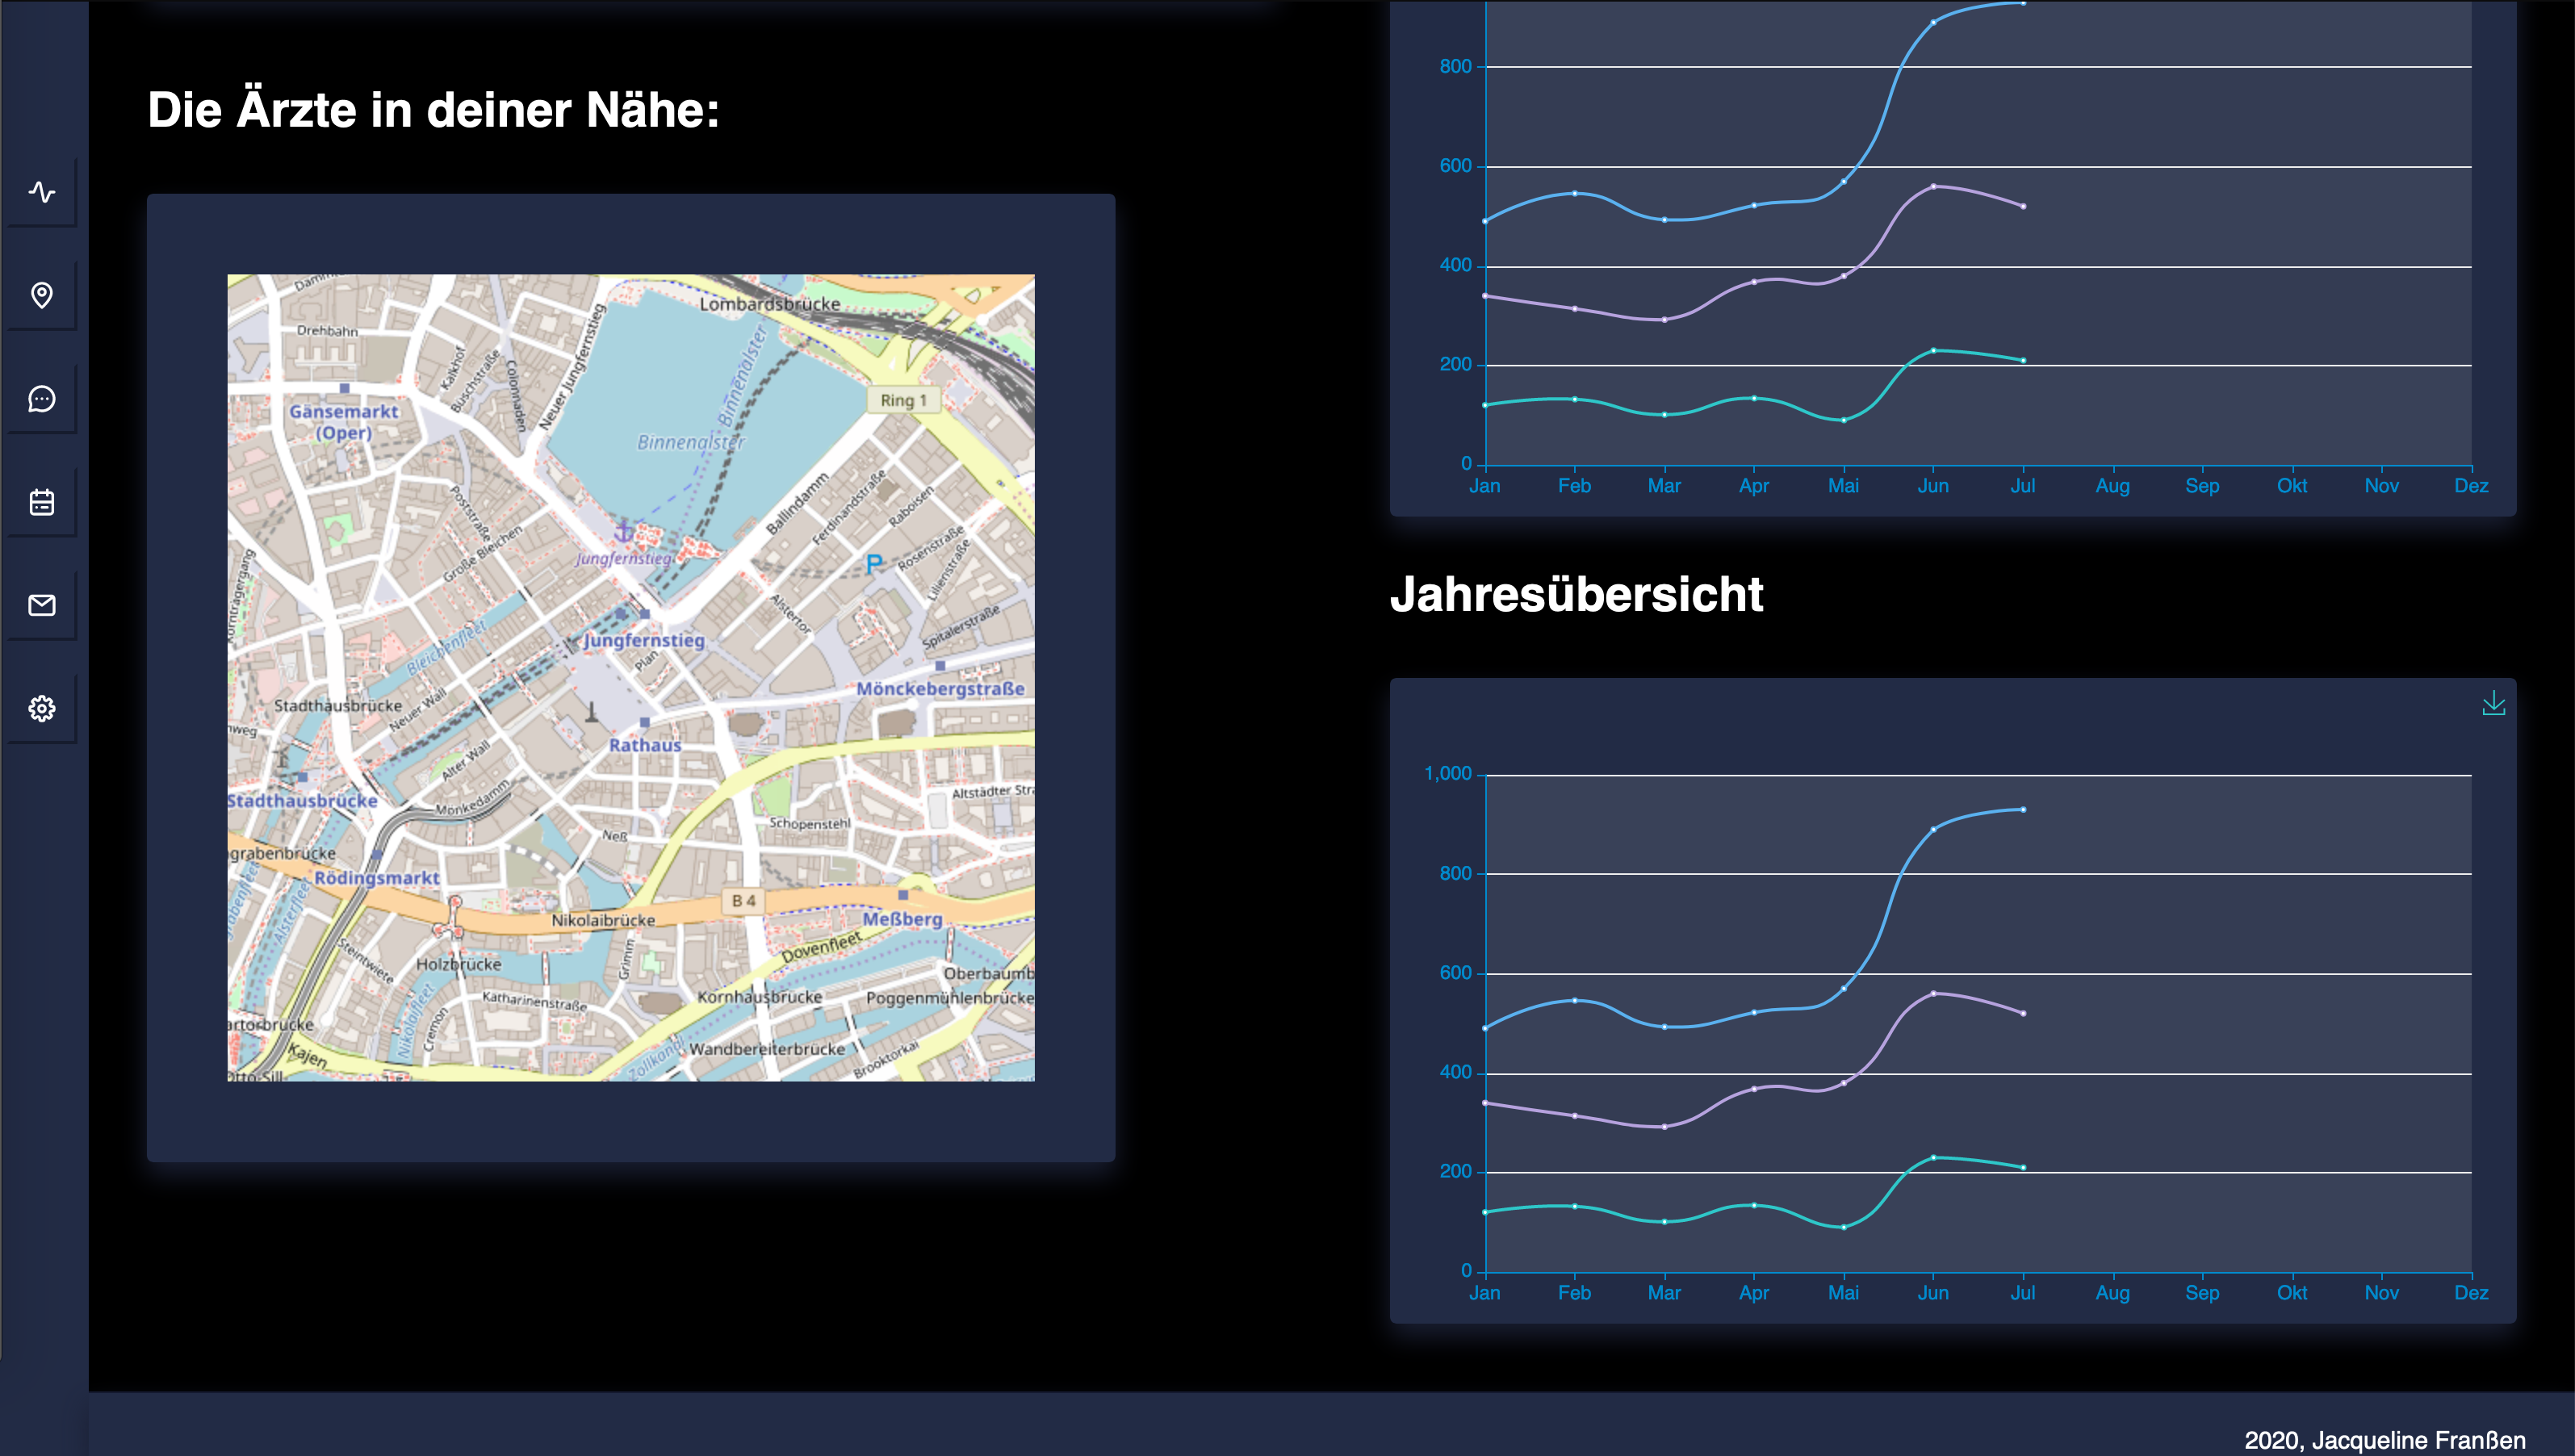
\includegraphics[width=1\textwidth]{images/angular_02.png}
	\caption{Angular Frontend (bottom page), map to show the nearest doctors}
	\label{angular_02}
\end{figure}

\paragraph{Connect Watson Assistant to Frontend}

To be able to connect to the Watson Assistant instance on IBM cloud, the API Version 2.0 had to be called. First of all, the current sessionId was requested to be able to interact with Watson Assistant. After that, a simple get request was executed to let the chatbot start the conversation. Everytime, the user sends a message to Watson Assistant, a post request is sent to the API and the response is the answer from Watson Assistant \footnote{cf.\autocite{wa_api_v2}}. In order to define the conversation's direction, the intent's probability is calculated (every intent has its own learning set which at least should include six sentences).

\paragraph{Data visualization: Development of a Python Script to show all measured values} 
\footnote{cf.\autocite{kaggle}}
\footnote{cf.\autocite{decision_tree_python}}


\paragraph{Development of recommendation of nearest doctors to patient}
outlook: maybe in future to connect to the doctors' calendar to directly make an appointment through the chatbot

\paragraph{Development of email service to send reports every two weeks to the doctor}

Another challenge was the way to automatically ask the user for his measured data. Most chatbot only helps in certain situations including precise user intents, e.g. the question 'When should i measure my blood pressure?'. By implementing a python script for data analysis an alarm was created to remind users every five hours or once a day.
In order to face this problem or use case, a routine including a timer had to be implemented.

\section{Problem solving}
\subsection{Tests}
\subsection{Dataset}
Since the setup of Watson Assistant API and the Angular Frontend took too much development time, a user test could not be executed. For that reason, the diagrams were calculated by using a dataset from Kaggle\footnote{cf.\autocite{kaggle}} which included 70000 entries of different patients and 12 characteristics. These 12 characteristics included:
\begin{itemize}
\setlength\itemsep{-0.5em}
  \item age (in days)
  \item gender
  \item height
  \item weight
  \item systolic value
  \item diastolic value
  \item cholesterol (1: normal, 2: above normal, 3: well above normal)
  \item gluc (1: normal, 2: above normal, 3: well above normal)
  \item smoke (binary)
  \item alco (binary)
  \item active (binary)
  \item presence or absence of cardiovascular disease (binary) 
\end{itemize}  


\section{Predictive Analytics: Creating a model to predict cardiovascular disease} \label{predict}
Generally, it is hard to let an algorithm diagnose cardiovascular disease if only looking at the dataset above. In practice, it needs the experience of a doctor and many different measured values in different situations (e.g. in stress situations or in relaxing situations). Nevertheless, for analytics it is very interesting to test if for example a neural network could learn on the given dataset and could predict the probability of a cardiovascular disease for a given patient. 

\subsection{Development of python script}

Based on the given Kaggle Dataset, a python script was developed. This script builds up a neural network for an intelligent and fast way to find out whether a person with given health characteristics has a higher or lower risk to suffer from cardiovascular disease.
Therefore during the first step of analysis the dataset had to be cleaned from null values and only the factors which are relevant for correlation analysis were used. All other values were eliminated. This was implemented by using seaborn's function 'heatmap'. The produced heatmap showed the parameters of the dataset and how they correlated with the classification variable 'cardio' (which means that the person suffers from cardiovascular disease or not).

As this is a binary classification problem sigmoid as the activation function was used.
Dense layer implements output = activation(dot(input, kernel) + bias). Kernel is the weight matrix. Kernel initialization defines the way to set the initial random weights of Keras layers.
To optimize the neural network an Adam function was used. Adam stands for Adaptive moment estimation and combines RMSProp and Momentum. Momentum takes the past gradients into account in order to smooth out the gradient descent.

\section{Results}

\chapter{Conclusion and Outlook }
\section{Conclusion}

\section{Outlook}


\subsection{Connect Flask app, python script and Angular frontend}

Figure \ref{architecture_perfect} shows the architecture which is aimed  

\begin{figure}[h]
	\centering
	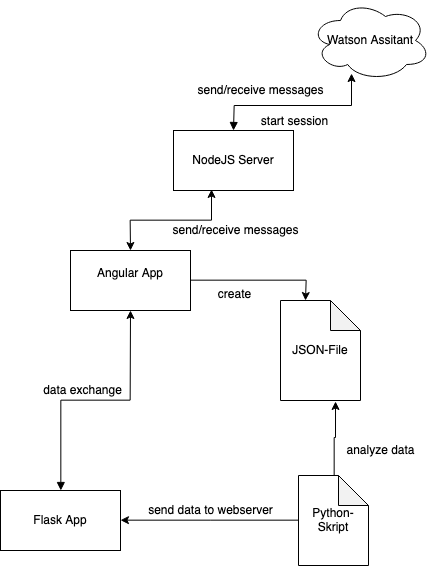
\includegraphics[width=1\textwidth]{images/architecture_perfectworld.png}
	\caption{Watson Assistant entitities}
	\label{architecture_perfect}
\end{figure}

Is a chatbot an appropriate solution for recording and reminding patients to measure their blood pressure ? 
In practice, most chatbots are created to solve and help multiple intents of their users and not to only 'retrieve' information.
On the one hand, the retrieved information can be used to run several analysis and to find out trends in the data. But on the other hand, the developed solution  supports users to never forget to measure and doctors to better understand trends in the measured data.
During development and research, there came up another issue: To inform patients precisely about their illness. Most patients go to doctors and describe their symptoms, the doctor makes some diagnosis and provides them some medication. But in most cases, doctors do not have enough time to answer all the questions of their patients. For that reason it might be useful to provide a 24/7 service for patients with chronic disease to both record their symptoms and measurements and to answer all their questions.


connection frontend (angularjs webpage) to mongodb through socket.io connection.
Connection between Watson Assistant and Frontend through mongodb and via socket.io connection.
\subsection{Behaviour change techniques}
\subsection{Therapy and Forecasting of healing}
As described in section \ref{predict}, a neural network can calculate the probability of a patient to suffer cardiovascular disease.
Moreover, another use case might be patients already suffering from cardiovascular disease which have to be treated and want to recover. In that situation the neural network could calculate the ideal weight,
It could provide personlaized nutrition plans. It could also forecast the term or maybe exact date (if trained well) when the patients will be healthy again and  

For future use cases, it might be very useful to have a proper dashboard for each doctor (which requires a user management and authentication mechanism) 

\subsection{Encrypt and save patient data}

It is important to store all measured and personal data in a secure way. Asynchronous encryption is a good way to save these data and to only allow access to the parties that should see the information, such as patients. To give an example, the application could save the data to the cloud and for this one action it uses a public key. If the patient wants to get to this information, he needs a private key to decrypt all information. 



\chapter{Abbreviations}
\begin{acronym}[ARIMA]
\acro{arima}[ARIMA]{Autoregressive Integrated Moving Average Model}
\acro{nlp}[NLP]{Natural Language Processing}
\acro{esarc}[ESARC]{Enterprise Software Architecture Reference Cube}
\acro{m-health}[M-HEALTH]{medical health}
\end{acronym}

\printbibliography[heading=bibintoc]

\chapter{Appendix A}\label{appendix a}
\ohead[]{Ehrenwörtliche Erklärung \hfill \thepage}

\null\vfill
\textbf{Ehrenwörtliche Erklärung}

Hiermit versichere ich, dass die vorliegende Arbeit von mir selbstständig und ohne unerlaubte Hilfe angefertigt worden ist, insbesondere dass ich alle Stellen, die wörtlich oder annähernd wörtlich aus Veröffentlichungen entnommen sind, durch Zitate als solche gekennzeichnet habe. Ich versichere auch, dass die von mir eingereichte schriftliche Version mit der digitalen Version übereinstimmt. Weiterhin erkläre ich, dass die Arbeit in gleicher oder ähnlicher Form noch keiner Prüfungsbehörde / Prüfungsstelle vorgelegen hat. Ich erkläre mich damit nicht einverstanden, dass die Arbeit der Öffentlichkeit zugänglich gemacht wird. Ich erkläre mich damit einverstanden, dass die Digitalversion dieser Arbeit zwecks Plagiatsprüfung auf die Server externer Anbieter hochgeladen werden darf. Die Plagiatsprüfung stellt keine Zurverfügungstellung für die Öffentlichkeit dar.

\ \\ \ \\ 


Ort, Datum (Vorname Nachname)

\vfill
\chapter{Appendix B}\label{appendix b}
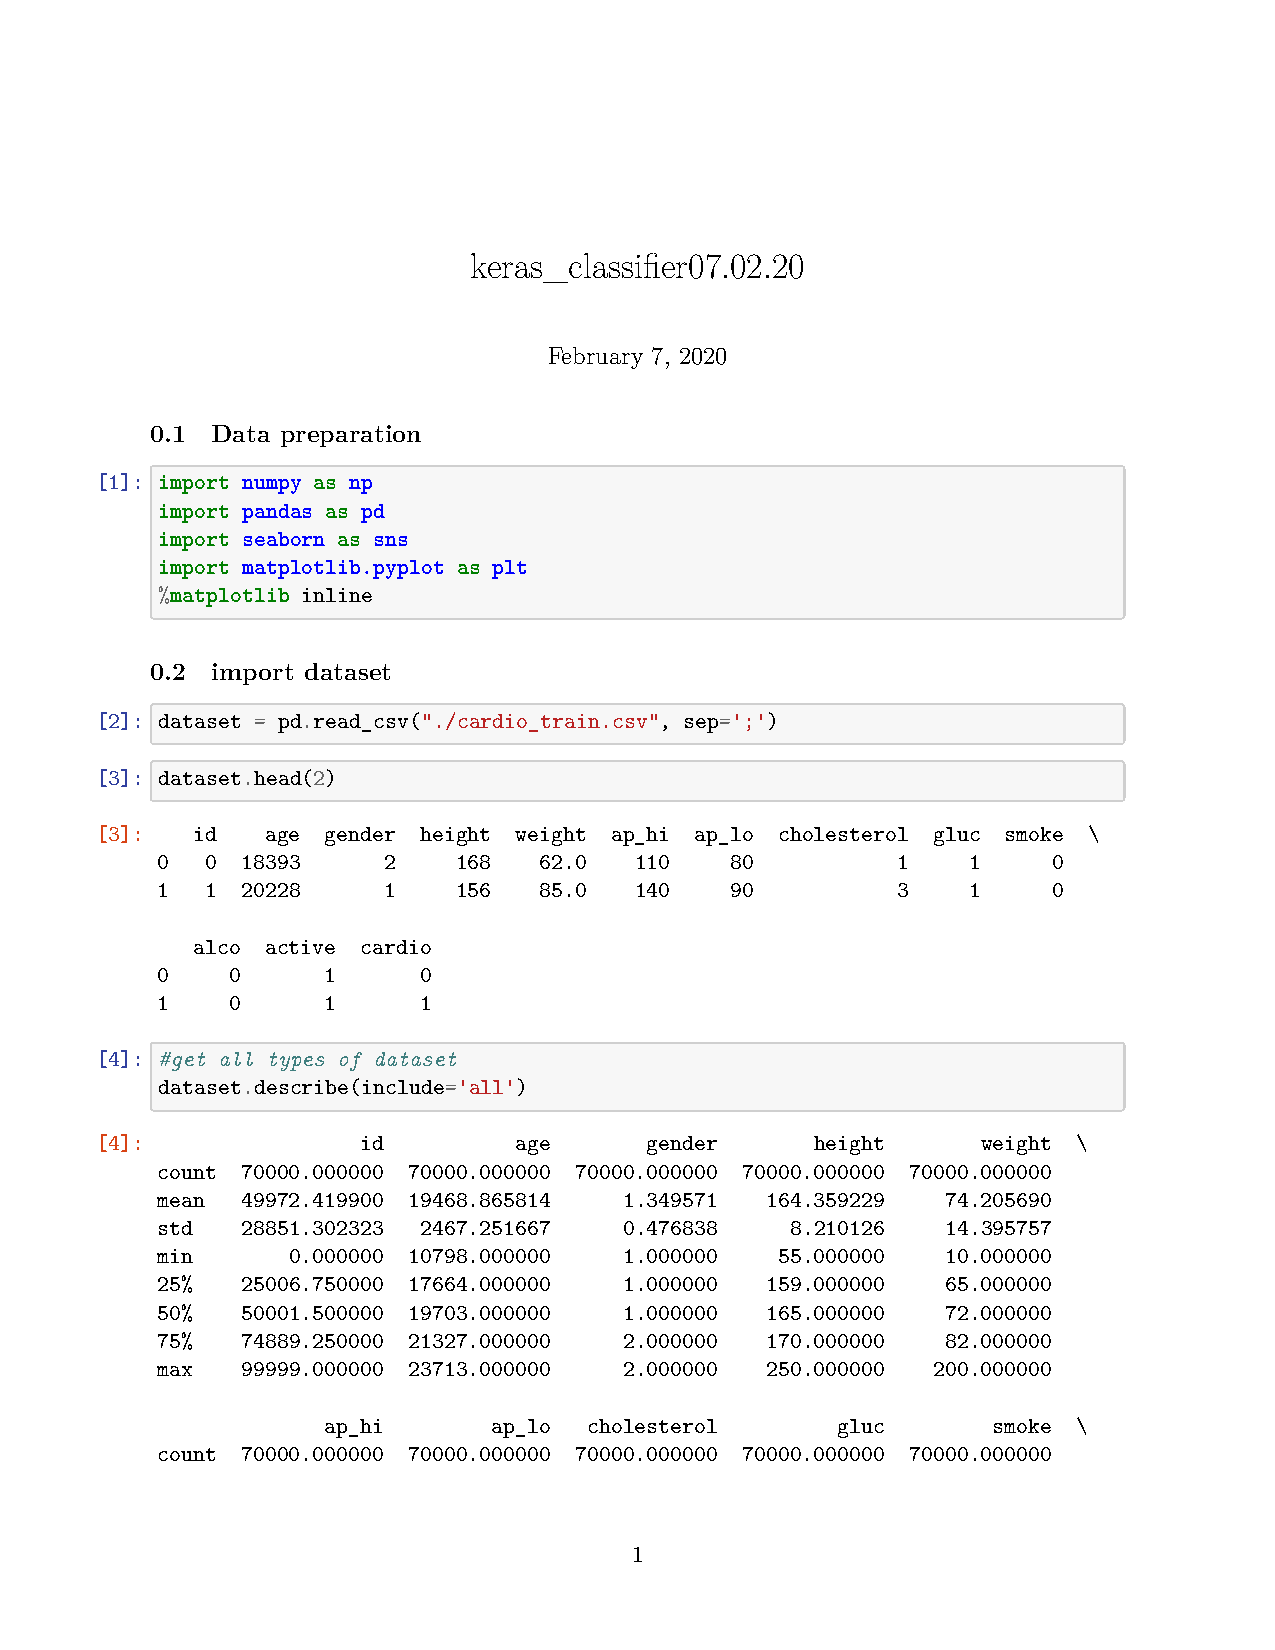
\includepdf[pages=-]{keras_classifier.pdf}

\end{document}
